% Copyright 2004 by Till Tantau <tantau@users.sourceforge.net>.
%
% In principle, this file can be redistributed and/or modified under
% the terms of the GNU Public License, version 2.
%
% However, this file is supposed to be a template to be modified
% for your own needs. For this reason, if you use this file as a
% template and not specifically distribute it as part of a another
% package/program, I grant the extra permission to freely copy and
% modify this file as you see fit and even to delete this copyright
% notice. 

\documentclass{beamer}
\usepackage[absolute,overlay]{textpos}
\usepackage[timeinterval=1]{tdclock}


\usepackage{amssymb,amsmath,amsfonts,amsthm}
\usepackage{url}
\usepackage[backend=bibtex,style=verbose]{biblatex}
%\footnotesize{\small}
\setbeamerfont{footnote}{size=\tiny}

\bibliography{s-arc-solCay.bib}

% There are many different themes available for Beamer. A comprehensive
% list with examples is given here:
% http://deic.uab.es/~iblanes/beamer_gallery/index_by_theme.html
% You can uncomment the themes below if you would like to use a different
% one:
%\usetheme{AnnArbor}
%\usetheme{Antibes}
%\usetheme{Bergen}
%\usetheme{Berkeley}
%\usetheme{Berlin}
%\usetheme{Boadilla}
%\usetheme{boxes}
%\usetheme{CambridgeUS}
%\usetheme{Copenhagen}
%\usetheme{Darmstadt}
%\usetheme{default}
%\usetheme{Frankfurt}
%usetheme{Goettingen}
%\usetheme{Hannover}
%\usetheme{Ilmenau}
%\usetheme{JuanLesPins}
%\usetheme{Luebeck}
\usetheme{Madrid}
%\usetheme{Malmoe}
%\usetheme{Marburg}
%\usetheme{Montpellier}
%\usetheme{PaloAlto}
%\usetheme{Pittsburgh}
%\usetheme{Rochester}
%\usetheme{Singapore}
%\usetheme{Szeged}
%\usetheme{Warsaw}


\usepackage{multirow}





\def\SL{\mathrm{SL}}
\def\GL{\mathrm{GL}}
\def\PSL{\mathrm{PSL}}
\def\PGL{\mathrm{PGL}}
\def\PSU{\mathrm{PSU}}
\def\PSp{\mathrm{PSp}}
\def\PO{\mathrm{P\Omega}}
\def\PGaL{\mathrm{P\Gamma L}}
\def\PSigU{\mathrm{P\Sigma U}}
\def\AGaL{\mathrm{A\Gamma L}}
\def\Aut{\mathrm{Aut}}
\def\Inn{\mathrm{Inn}}
\def\Out{\mathrm{Out}}
\def\Cay{\mathrm{Cay}}
\def\val{\mathrm{val}}
\def\HS{\mathrm{HS}}
\def\PH{\mathcal{PH}}
\def\GI{\mathcal{GI}}
\def\PG{\mathrm{PG}}
\def\soc{\mathrm{soc}}
\def\proof#1{\textbf{Proof.}{#1}\qed}


\def\TWthm{\begin{theorem}[2.2, Thompson-Wielandt]
Let $\Gamma$ be a connected $(G, s)$-transitive graph with $s\geq  2$, and let $\alpha$ and $\beta$ be adjacent vertices of $\Gamma$. Then one of the following holds, where p is a prime:
\begin{enumerate}
	\item $s\leq 3$, $G_{\alpha\beta}^{[1]}=1$, and $G_{\alpha}^{[1]}\cong(G_{\alpha}^{[1]})^{\Gamma(\beta)}\triangleleft G_{\alpha\beta}^{\Gamma(\beta)}\cong G_{\alpha\beta}^{\Gamma(\alpha)}$;
	\item $s\leq 3$, $G_{\alpha\beta}^{[1]}$ is a nontrivial p-group, $\PSL_d(p^f)\triangleleft G_\alpha^{\Gamma(\alpha)}$ for some $d\geq 2$, and $\val(\Gamma)=(p^{df}-1)/(p^f-1)$;
	\item $s\geq 4$, $\PGL_2(p^f)\triangleleft G_\alpha^{\Gamma(\alpha)}$, $\val(\Gamma)=p^f+1$, and one of the following occurs:
	\begin{enumerate}[i]
		\item s=4, and $G_\alpha=p^{2f}:\frac{p^f-1}{(3,p^f-1)}.\PGL_2(p^f).\mathcal{O}$ with $|\mathcal{O}|\mid (3,p^f-1)f$;
		\item s=5, and $G_\alpha=p^{3f}:\GL_2(2^f).\mathbb{Z}_e$ with $e|f$;
		\item s=7, and $G_\alpha=(p^{2f}\times (p^f)^{1+2}):\GL_2(3^f).\mathbb{Z}_e$ with $e|f$.
	\end{enumerate}
\end{enumerate}
\end{theorem}}

\def\LemThree{\begin{lemma}[2.3]
For a connected $(G,3)$-arc-transitive graph $\Gamma$ and adjacent vertices $\alpha,\beta$, at least one of the following holds: \footcite{LI2015331}\textsuperscript{,Thm 4.2}
\begin{enumerate}
	\item $G_\alpha^{[1]}$ is transitive on $\Gamma(b)\backslash\{\alpha\}$.
	\item $G_\alpha=A_7$ or $S_7$.
	\item $\mathbb{Z}_p^f\triangleleft G_\alpha^{\Gamma(\alpha)}\leq \AGaL_1(p^f)$ with p a prime.
\end{enumerate}
\end{lemma}}


\def\LemFive{\begin{lemma}[2.5]
Let $\Gamma$ be a connected $(G,s)$-transitive graph with $s\geq 3$, and suppose $N\triangleleft G$ and not semiregular. Then one of the following holds:
\begin{enumerate}
	\item both $G_\alpha^{\Gamma(\alpha)}$ and $N_\alpha^{\Gamma(\alpha)}$ are almost simple 2-transitive;
	\item $G_\alpha^{\Gamma(\alpha)}$ is affine and $N_\alpha^{\Gamma(\alpha)}$ is primitive.
\end{enumerate}
\end{lemma}}


\newtheorem{proposition}{Proposition}[theorem]


%%%%%%%%%%

%START

%%%%%%%%%%








\begin{document}


\title{s-Arc-transitive solvable Cayley graphs}
\setbeamerfont{subtitle}{size=\fontsize{8}{15}}
\subtitle{CAI HENG LI, JIANGMIN PAN, AND YINGNAN ZHANG}

% A subtitle is optional and this may be deleted
%\subtitle{PhD Thesis Defense}

\author{Speaker: Yuandong Li}
% - Give the names in the same order as the appear in the paper.
% - Use the \inst{?} command only if the authors have different
%   affiliation.

\institute[BJTU] % (optional, but mostly needed)
{Beijing Jiaotong University}

% - Use the \inst command only if there are several affiliations.
% - Keep it simple, no one is interested in your street address.

\date{\today}
% - Either use conference name or its abbreviation.
% - Not really informative to the audience, more for people (including
%   yourself) who are reading the slides online

%\subject{Applied Math}
% This is only inserted into the PDF information catalog. Can be left
% out. 

% If you have a file called "university-logo-filename.xxx", where xxx
% is a graphic format that can be processed by latex or pdflatex,
% resp., then you can add a logo as follows:

% \pgfdeclareimage[height=0.5cm]{university-logo}{university-logo-filename}
% \logo{\pgfuseimage{university-logo}}

% Delete this, if you do not want the table of contents to pop up at
% t`	he beginning of each subsection:
\AtBeginSubsection[]
{
  \begin{frame}<beamer>{Outline}
    \tableofcontents[currentsection,currentsubsection]
  \end{frame}
}




% Let's get started


\begin{frame}
\titlepage
%\initclock
%\date[\initclock \cronominutes\timeseparator\cronoseconds]{}
\end{frame}
\date{\crono}


\begin{frame}{Outline}
 \tableofcontents
\end{frame}

% Section and subsections will appear in the presentation overview
% and table of contents.


\section{Preliminaries \& Background}

\begin{frame}{Preliminaries}
Let $\Gamma$ be a finite simple undirected graph. Let $G\leq \Aut\Gamma$.
\begin{definition}
	\begin{itemize}
		\item \textbf{s-arc:} (s+1)-tuple of vertices $\alpha_0,\alpha_1,\cdots,\alpha_s$ where $\alpha_i$ is adjacent to $\alpha_{i+1}$ and $\alpha_{j-1}\neq\alpha_{j+1}$ for $0\leq i\leq s-1$ and $1\leq j\leq s-1$.
		\item \textbf{(G,s)-arc-transitive:} $G$ is transitive on the set of s-arcs of $\Gamma$.
		\item \textbf{(G,s)-transitive:} (G,s)-arc-transitive but not (G,s+1)-arc-transitive.
	\end{itemize}
For short, \textbf{s-transitive} means $(\Aut\Gamma,s)$-transitive for graphs.
\end{definition}
\begin{lemma}
	\begin{itemize}
		\item s-arc-transitive ($1\leq s$) $\Longrightarrow$ k-arc-transitive ($1\leq k\leq s$).
		\item the s-arc-transitivity of a graph is inherited by the normal quotients.
	\end{itemize} 
\end{lemma}
\end{frame}

\begin{frame}{Preliminaries}
\begin{definition}
	\begin{itemize}
		\item \textbf{Cayley graph:} $\Cay(G,S)$ with vertex set $G$ and edges $yx^{-1}\in S$.
		\item \textbf{solvable Cayley graph:} $G$ is solvable.
	\end{itemize}
\end{definition}
\begin{lemma}
	\center $\Gamma$ is Cayley of $G$ $\iff$ $\exists G\lesssim \Aut\Gamma$ which is vertex-regular.
\end{lemma}
\end{frame}

\begin{frame}{Preliminaries}
\begin{definition}
	A transitive permutation group G is said to be \\\textbf{quasiprimitive} if its nontrivial normal subgroups are transitive, and \\\textbf{bi-quasiprimitive} if its nontrivial normal subgroups have at most 2 orbits and there exists one which has exactly 2 orbits.
\end{definition}

The O'Nan-Scott-Praeger theorem \footcite{praeger_1997} divides the quasiprimitive permutation groups into 8 types: holomorph affine (HA), holomorph simple (HS), holomorph compound (HC), almost simple (AS), simple diagonal (SD), compound diagonal (CD), product action (PA) and twisted wreath product (TW).
\end{frame}


\begin{frame}{Background}
\begin{itemize}
	\item 1947, Tutte: No 6-arc-transitive trivalent graphs.
	\item 1981, Weiss: No s-arc-transitive graphs with $\val\geq 3$ for $s=6$ and $s\geq 8$.
	\item 2019, Li C.H. \& Xia B.Z.: \\ Connected \textbf{non-bipartite} 3-arc-transitive solvable Cayley graph with $\val\geq 3$ is a normal cover of the Hoffman-Singleton graph or the Petersen graph.
	\item 2021, Zhou J.X.: No such normal covers, so $s\leq 2$ sharply.
\end{itemize}

\begin{problem}
Studying connected \textbf{bipartite} s-arc-transitive solvable Cayley graphs, and determining the upper bound on $s$.	
\end{problem}
For convenience, one may assume $s\geq 3$ and $\val\geq 3$. 

\end{frame}




\section{Main Result \& Examples}
\begin{frame}{Main Result}
\begin{theorem}
Every connected s-arc-transitive solvable Cayley graph with $s\geq 3$ and $val\geq 3$ is a normal cover of one of the following graphs:	
\begin{enumerate}
	\item the complete bipartite graph $K_{n,n}$ with $n\geq 3$;
	\item the geometry incidence graph $\mathcal{GI}(5, 2, 2)$;
	\item the standard double cover of the Hoffman-Singleton graph;
	\item a graph $\Sigma$ with valency $p^f+1$ such that $\PSL_3(p^f).2\leq \Aut\Sigma\leq \Aut(\PSL_3(p^f))$ and $\mathbb{Z}_p^{2f}:\SL_2(p^f)\triangleleft(\Aut\Sigma)_\alpha$, where $p^f\geq 3$ is a prime power and $\alpha$ is a vertex.
\end{enumerate}
In particular, the sharp upper bound on s is 4.
\end{theorem}
These normal covers are being investigated in a sequel. (usually challenge)
\end{frame}

\begin{frame}{Examples}
(1) $\mathbf{K}_{n,n}$ with $n\geq 3$
\begin{itemize}
	\item 3-transitive
	\item $\mathbf{K}_{n,n}\cong \Cay(G,G\backslash H)$ where $G$ is solvable and $H<G$ of index 2
\end{itemize}

(2) $\mathcal{GI}(5,2,2)$
\begin{itemize}
	\item the incidence graph of $(\mathcal{P,L})$ where $\mathcal{P}$(resp. $\mathcal{L}$) is the set of 2-subspace(resp. 3-subspace) of $\mathbb{F}_2^5$
	\item $\Aut(\GI(5,2,2))=\GL_5(2).\langle \sigma\rangle$ is vertex-transitive
	\item $G_\alpha=2^6:(\GL_2(2)\times\GL_3(2))$, $G_{\alpha\beta}=2^8:(S_3\times S_3)$, val=$\frac{|G_\alpha|}{|G_{\alpha\beta}|}$=7
	\item 3-transitive\footcite{LI20162907}$^\text{,Theorem 3.4}$
	\item $G=RG_\alpha$ with $R\cong 31:5:2$ vertex-regular\footcite{LI2022factorizations}$^\text{, Theorem 1.1}$
\end{itemize}

\end{frame}

\begin{frame}{Examples}
(3) $\HS_{50}^{(2)}$
\begin{itemize}
	\item $\HS_{50}$ is 3-transitive \\$\Aut(\HS_{50})=\PSigU(3,5)$ has a solvable vertex-transitive subgroup\\ It is NOT a Cayley graph
	\item \textbf{standard double cover:} $\Gamma^{(2)}=(\tilde{V},\tilde{E})$ of $\Gamma=(V,E)$, where\\ $\tilde{V}=V\times\{1,2\}$, $\tilde{E}=\{\{(v,1),(w,2)\}\mid\{v,w\}\in E\}$\\ $\Aut(\Gamma^{(2)})\geq \Aut\Gamma\times\langle\sigma\rangle$, $\Gamma$ s-arc-transitive $\implies$ $\Gamma^{(2)}$ s-arc-transitive
	\item By MAGMA, $\exists_1$ connected $G$-arc-transitive 7-valent graph $\Gamma$ of order 50 with $(G,G_\alpha)=(\PSU_3(5),A_7)$ or $(\PSU_3(5).\mathbb{Z}_2,S_7)$. $\Gamma\cong \HS_{50}$
	\item By MAGMA, $\exists_1$ connected $G$-arc-transitive 7-valent graph $\Gamma$ of order 100 with $(G,G_\alpha)=(\PSU_3(5).\mathbb{Z}_2,A_7)$. $\Gamma\cong \HS_{50}^{(2)}$
\end{itemize}
(\textcolor{red}{Q: Could a normal cover of $\HS_{50}^{(2)}$ be solvable Cayley?} see Zhou's paper)
\end{frame}

\begin{frame}{Examples}
(4) $\mathcal{PH}(3,q)$
\begin{itemize}
	\item the incidence graph of $\PG(2,q)=(\mathcal{P,L})$, where \\$\mathcal{P}$(resp. $\mathcal{L}$) is the set of 1-subspace(resp. 2-subspace) of $\mathbb{F}_q^3$
	\item $\Aut(\PH(3,q))=\PGaL_3(q).\langle \sigma\rangle=\Aut(\PSL_3(q))$
	\item $(\alpha_0,\cdots,\alpha_4)$ with $\alpha_0\in \mathcal{P}$ corresponds to a basis $v_1,v_2,v_3$ such that\[ \alpha_0=\langle v_1\rangle, \alpha_1=\langle v_1,v_2\rangle, \alpha_2=\langle v_2\rangle, \alpha_3=\langle v_2,v_3\rangle, \alpha_4=\langle v_3\rangle \]all ordered bases are equiv. under linear transformation\\$\implies$ 4-arc-transitive
	\item a Cayley graph\footcite{MARUSIC2003162} of $D_{2(q^2+q+1)}$, for example Heawood graph.
\end{itemize}
\end{frame}


\section{Proof of the Main result}

\subsection{Overview of the proof}

\begin{frame}{Overview of the proof}
	Let $\Gamma=\Cay(H,S)$ be connected, $(G,s)$-transitive, $\val\geq 3$,\\ with $H$ solvable, $H\leq G\leq \Aut\Gamma$, $s\geq 3$.
	
	Let $M\triangleleft G$ (may trivial) be maximal with $\geq 3$ orbits on $V\Gamma$.\\Then
	\begin{itemize}
		\item $\Gamma$ is a normal cover of $\Gamma_M$
		\item $\Gamma_M$ is $(G/M,s)$-arc-transitive
		\item $G/M$ is either quasiprimitive or bi-quasiprimitive on $V\Gamma_M$, $|V\Gamma_M|\geq 3$
	\end{itemize}

\begin{theorem}[Praeger,1993]
Let $\Gamma$ be a finite connected graph, $G\leq \Aut\Gamma$ is s-arc transitive on $\Gamma$ for some $s\geq 2$. Suppose $N\triangleleft G$ has more than two orbits on vertices. Then\begin{enumerate}
	\item $\Gamma_N$ is finite and connected and the group of automorphisms of $\Gamma_N$ induced by G is s-arc transitive on $\Gamma_N$.
	\item N is semiregular on vertices (that is $N_\alpha= 1$ for each vertex $\alpha$ of $\Gamma$) and $\Gamma$ is a cover of $\Gamma_N$. 
\end{enumerate}  
\end{theorem}

\end{frame}

\begin{frame}{Overview of the proof}
\textbf{Case quasiprimitive:} 
$\Gamma_M$ non-bipartite. By Li-Xia-Zhou, no such graphs.

\textbf{Case bi-quasiprimitive:} $\Gamma_M$ bipartite.

Then either $\Gamma_M=\mathbf{K}_{n,n}$, or $G/M$ is almost simple. \textcolor{blue}{(Reduce to AS type)}\\Moreover, $\soc(G/M)$ is a classical simple group of Lie type. \\\textcolor{blue}{(Use factorization of AS groups with a solvable factor)}

\ 

Let $s_0$ be the sharp upper bound on $s$.
\begin{itemize}
	\item By Example (4), $\PH(3,q)$ is 4-transitive, so $s_0\geq 4$.
	\item If there is a connected 5-arc-transitive solvable Cayley graph $\Gamma$, \\ then $\Gamma$ is a normal cover of a 5-arc-transitive graph of type (1)-(4),\\ while analysis above states no such graph. 
\end{itemize}
Hence $s_0=4$.
\end{frame}

\subsection{Reduce to almost simple groups} 
\begin{frame}{Reduce to almost simple groups}
In the remains of this talk, we assume the followings.

\begin{itemize}
	\item Let $\Gamma$ be a connected bipartite $(G,s)$-transitive graphs of val$\geq 3$, with bipartitions $\Delta_1$ and $\Delta_2$ and $s\geq 3$.
	\item Suppose $G$ is bi-quasiprimitive on $V\Gamma$ and contains a vertex-transitive solvable subgroup $H$. 
	\item Set $G^+=G_{\Delta_1}$, the setwise stabilizer of $G$ on $\Delta_1$, and $H^+=H\cap G^+$.
	\item Let $\alpha$, $\beta$ be adjacent vertices.
\end{itemize}

Some immediate facts:
\begin{itemize}
	\item $G^+=G_{\Delta_1}=G_{\Delta_2}$ has index 2 (hence normal) in $G$ and is transitive on both $\Delta_1$ and $\Delta_2$, as well as $H^+$ in $H$.
	\item $G=\langle G^+,g\rangle$ where $g\in G\backslash G^+$, $g$ interchanges $\Delta_1$ and $\Delta_2$, $g^2\in G^+$
\end{itemize}

\end{frame}


\begin{frame}{Case: unfaithful action}
Now we consider the action of $G^+$ on $\Delta_1$ and $\Delta_2$.
\begin{lemma}[4.2]
	If $G^+$ acts unfaithfully on $\Delta_1$ or $\Delta_2$, then $\Gamma=\mathbf{K}_{n,n}$, where $n=|V\Gamma |/2$.
\end{lemma}
\proof{
Let $K=\ker(G^+\curvearrowright\Delta_1)$. \\Then $K^g=\ker(G^+\curvearrowright\Delta_2)$ and $1\neq KK^g=K\times K^g\triangleleft G$.\\$\because$ $G$ is bi-quasiprimitive, $K\times K^g$ has at most 2 orbits.\\Since $K^g$ fixes $\Delta_2$ pointwise, $K$ must be transitive on $\Delta_2$.\\It follows that $\Gamma=\mathbf{K}_{n,n}$.}

\ 

We thus additionally assume $G^+$ is faithful on both $\Delta_1$ and $\Delta_2$.\[G^+\cong (G^+)^{\Delta_1}\cong (G^+)^{\Delta_2}\]
We will prove the above actions are quasiprimitive of almost simple type.
\end{frame}

\begin{frame}{Quasiprimitive $\implies$ same type AS or PA}
\begin{lemma}[4.3]
	Suppose $G^+$ is quasiprimitive on $\Delta_1$ or $\Delta_2$. Then \begin{enumerate}
		\item $G^+$ is quasiprimitive on both $\Delta_1$ and $\Delta_2$
		\item both $ (G^+)^{\Delta_1}$ and $ (G^+)^{\Delta_2}$ have the same type AS or PA
	\end{enumerate}
\end{lemma}
\proof{WLOG, assume $G^+$ is quasiprimitive on $\Delta_1$.\\$G$ transitive on $V\Gamma$ and $G^+\triangleleft G$ $\implies$ $G^+\curvearrowright\Delta_1$, $\Delta_2$ are perm. isom.\\Hence $G^+$ is quasiprimitive on $\Delta_2$ of the same type on $\Delta_1$.\\By ref.\footcite{GIUDICI2003analysing}\textsuperscript{,Thm 1.2}, $(G^+)^{\Delta_1}$ is of type HA, AS, TW or PA.\\For cases HA or TW, $\soc(G^+)\triangleleft G$ is regular on $\Delta_1$ and $\Delta_2$, \\then $\Gamma$ is a \textbf{G-normal bi-Cayley graph} on $\soc(G^+)$.\\By ref.\footcite{CONDER2020264}\textsuperscript{,Lem 3.2}, $\Gamma$ is at most $(G,2)$-arc-transitive, contradicting $s\geq 3$.}%\\Thereby, $G^+$ has the same type AS or PA on $\Delta_1$ and $\Delta_2$.}
\end{frame}


\begin{frame}{Study $\soc(G^+)$}
\begin{lemma}[4.4]
$\soc(G^+)$ is nonsolvable and is the the unique minimal normal subgroup of $G$, and $\soc(G^+)_\alpha\neq 1$.
\end{lemma}
\textbf{Proof.}{\\ If $G^+\curvearrowright\Delta_1$ is quasiprimitive. \\By lemma 4.3, $G^+$ is of type AS or PA.\\So $\soc(G^+)\mathop{\triangleleft}\limits_{min}G^+$ and is nonsolvable and not semiregular.\\ Let $C=C_G(\soc(G^+))$. Then $C\triangleleft G$ and $\soc(G^+)\cap C=Z(\soc(G^+))=1$.\\If $C\neq 1$, as $C\cap G^+=1$ and $G=G^+.2$, we derive that $C\cong \mathbb{Z}_2$.\\ Since $|V\Gamma|>4$, C has more than 2 orbits, contradicting G bi-quasiprimitive.\\Hence $C=1$ and $\soc(G^+)$ is also unique in $G$.
}
\end{frame}

\begin{frame}
Now assume $G^+$ is not quasiprimitive on both $\Delta_1$ and $\Delta_2$.\\ Then $\exists M\mathop{\triangleleft}\limits_{min} G^+$ acting intransitively on $\Delta_1$ hence has $> 2$ orbits on $V\Gamma$. Thus $M\not\triangleleft G$ and $M^g\neq M$. (Recall $G=\langle G^+,g\rangle$)\\Since $g^2\in G^+$, one has $MM^g=M\times M^g\leq G^+$ is normal in $G$.\\By bi-quasiprimitivity of $G$, $M\times M^g$ is transitive on $\Delta_1$ and $\Delta_2$.

By ref.\footcite{LI2002197}\textsuperscript{,Thm 1.5}, either
\begin{enumerate}[(a)]
	\item $M\times M^g$ is regular on $\Delta_1$ and $\Delta_2$; or
	\item $\soc(G^+)=M\times M^g$ is nonsolvable and not semiregular, and is the unique minimal normal subgroup of G.
\end{enumerate}
For case (b), done.\\
For case (a), $\Gamma$ is a G-normal bi-Cayley graph on $M\times M^g$, again by ref.\footcite{CONDER2020264}\textsuperscript{,Lem 3.2}, is at most $(G,2)$-arc-transitive. A contradiction.\qed 
\end{frame}


\begin{frame}{Structure of $\soc(G^+)$}
According to Lemma 4.4, we may set that
\[ N:=\soc(G^+)=T_1\times T_2\times\cdots\times T_d\cong T^d\mathop{\triangleleft}\limits_{min}^{unique} G . \]
Then $N$ is transitive on $\Delta_1$ and $\Delta_2$ since $G$ is bi-quasiprimitive.

\ 

Consider $G^+\curvearrowright \{T_1,\cdots,T_d\}$ by conjugation with kernel $K$.

Then $N\triangleleft K\leq \Aut(T_1)\times \cdots\times \Aut(T_d)$. 
And $T_j\triangleleft K$, $1\leq j\leq d$. 

Let $M_j=C_K(T_j)$. Then\[ \cdots\times T_{j-1}\times 1\times T_{j+1}\times \cdots\leq M_j\leq \cdots\times \Aut(T_{j-1})\times 1\times  \Aut(T_{j+1})\times \cdots \]
$M_j\triangleleft K$ and $K/M_j\lesssim \Aut(T_j)$ is almost simple with socle $T_j$.%\\A subgroup of $K$ is called \textbf{diagonal} if it is isomorphic to its projection on $\Aut(T_j)$ for each $1\leq j\leq d$.

\ 

Recall $H$ is a vertex-transitive solvable subgroup of $G$. 

Let $H^+=H\cap G^+$ and $H_j$ be the projection of $H^+\cap N$ on $T_j$, $1\leq j\leq d$.

Then $|H^+\cap N|$ divides $|H_1||H_2|\cdots|H_d|$.

\end{frame}



\begin{frame}{Exclude PA type}
\begin{lemma}[4.5]
Suppose $d\geq 2$. Then $\exists j\in\{1,2,...,d\}$ s.t. $M_j$ is transitive on $\Delta_1$ or $\Delta_2$; in particular, if $G^+$ is quasiprimitive on $\Delta_1$ or $\Delta_2$, then it is not of type PA.
\end{lemma}
\textbf{Proof. }\\
Assume $G^+$ is quasiprimitive of type PA on $\Delta_1$ or $\Delta_2$. \\
Then $\exists \mathcal{B}=\Omega^d$ a maximal block system s.t. $G^+\curvearrowright\mathcal{B}$ primitive by PA.\\
For $(w_1,w_2,...,w_d)\in\Omega^d$, $(x_1,x_2,...,x_d)\in M_j$, we have
\[(w_1,w_2,...,w_d)^{(x_1,x_2,...,x_d)}=(w_1^{x_1},w_2^{x_2},...,w_d^{x_d}).\]
From previous analysis, $x_j=1$. Then transitivity of $M_j$ implies $|\Omega|=1$.\\
\textcolor{blue}{Need to prove the transitivity of some $M_j$.}
\end{frame}

\begin{frame}
Before that we prepare some lemmas.
\TWthm
\end{frame}

\begin{frame}
\LemThree


\LemFive
\end{frame}

\begin{frame}
\textbf{Proof of Lemma 2.5:}
\begin{itemize}
	\item $(G,3)$-arc-transitive $\implies$ $G_\alpha^{\Gamma(\alpha)}$ is 2-transitive (AS or affine)
	\item $N\triangleleft G$, $N_\alpha\neq 1$ and connectivity $\implies$ $1\neq N_\alpha^{\Gamma(\alpha)}\triangleleft G_\alpha^{\Gamma(\alpha)}$ transitive
\end{itemize}



\underline{Claim: }
\[G_{\alpha\beta}^{[1]}=1\text{ and }G_\alpha^{[1]}\curvearrowright\Gamma(\beta)\backslash\{\alpha\}\text{ transitive }\implies\ N_\alpha\curvearrowright \Gamma(\alpha)\text{ 2-transitive}\]
\begin{itemize}
	\item check $G_\beta^{[1]}/G_{\alpha\beta}^{[1]}\cong(G_\beta^{[1]})^{\Gamma(\alpha)}\triangleleft N_{\alpha\beta}^{\Gamma(\alpha)}$
	\item $G_\beta^{[1]}$ (hence $N_{\alpha\beta}$) $\curvearrowright \Gamma(\alpha)\backslash\{\beta\}$ transitive
\end{itemize}

\textcolor{red}{Better change the conditions to $G_{\alpha\beta}^{[1]}=1$ and 3-arc-transitive?}
\end{frame}


\begin{frame}
\textbf{$G_\alpha^{\Gamma(\alpha)}$ AS:}\\
By ref.\footcite{Cameron1981}\textsuperscript{, Thm5.3(S)Notes(2)}, either $N_\alpha^{\Gamma(\alpha)}$ is 2-transitive, or $N_\alpha^{\Gamma(\alpha)}=\PSL_2(8)$ primitive with $\val(\Gamma)=28$. The latter one is impossible.

\ 

\textbf{$G_\alpha^{\Gamma(\alpha)}$ affine:}
\begin{enumerate}
	\item $s\geq 4$:
		\begin{enumerate}
			\item $\val(\Gamma)=3$, $N_\alpha^{\Gamma(\alpha)}\geq \mathbb{Z}_3$ primitive 
			\item $\val(\Gamma)=4$ and $G_\alpha^{\Gamma(\alpha)}=\PGL_2(3)\cong S_4$, 
				\begin{enumerate}
					\item $N_\alpha^{\Gamma(\alpha)}=A_4$ or $S_4$ is 2-transitive
					\item $N_\alpha^{\Gamma(\alpha)}\cong\mathbb{Z}_2^2$ is regular, $N_{\alpha\beta}\curvearrowright \Gamma(\alpha)\cup\Gamma(\beta)$ trivial, connect $\implies$ $N_{\alpha\beta}=1$, hence $N_\alpha=\mathbb{Z}_2^2$, but by ref.\footcite{LI2006164}\textsuperscript{, lem 2.5}, no such normal subgroup
				\end{enumerate}
		\end{enumerate}
	\item $s=3$: $\mathop{\implies}\limits^{Thm 2.2} G_{\alpha\beta}^{[1]}=1$. Consider $G_\alpha^{[1]}\curvearrowright\Gamma(\beta)\backslash\{\alpha\}$
		\begin{itemize}
			\item[trans] $\mathop{\implies}\limits^{Claim} N_\alpha^{\Gamma(\alpha)}$ 2-transitive
			\item[intrans.] $\mathop{\implies}\limits^{lem 2.3}\mathbb{Z}_p^f\triangleleft G_\alpha^{\Gamma(\alpha)}\leq\AGaL_1(p^f)$, so $G_\beta^{[1]}\cong(G_\beta^{[1]})^{\Gamma(\alpha)}\triangleleft G_{\alpha\beta}^{\Gamma(\alpha)}\leq \mathbb{Z}_{p^f-1}.\mathbb{Z}_f$\\but this leads to a contradiction.\qed
		\end{itemize}
\end{enumerate}
\end{frame}

\begin{frame}
\LemFive
By lemma 4.4, $N\triangleleft G$ and $N_\alpha\neq 1$, $\forall \alpha\in V\Gamma$. 

Applying lemma 2.5, we have $\Gamma$ is $N$-locally-primitive.

Hence \textcolor{blue}{$\Gamma$ is $K$-locally-primitive} since $N\leq K$.

\end{frame}


\begin{frame}
\begin{lemma}[2.4]
Let $\Gamma$ be a connected bipartite G-locally-primitive graph with G-orbits $\Delta_1$ and $\Delta_2$ on $V\Gamma$ and each $|\Delta_i|>1$. Suppose $\exists N\triangleleft G$ s.t. N is intransitive on $\Delta_1$ and $\Delta_2$. Then \footcite{GIUDICI2003analysing}\textsuperscript{,Lem 5.1}
\begin{enumerate}
	\item $\Gamma$ is a normal cover of $\Gamma_N$.
	\item $N$ is semiregular on $V\Gamma$, $G^{V\Gamma_N}\cong G/N$ and $G_\alpha\cong(G/N)_v$ for $\alpha\in V\Gamma$ and $v\in V\Gamma_N$.
	\item $\Gamma_N$ is $G/N$-locally-primitive. Futhermore, if $\Gamma$ is locally $(G,s)$-arc- transitive with $s\geq 2$, then $\Gamma_N$ is locally $(G/N,s)$-arc-transitive.
\end{enumerate}
\end{lemma}
If $M_j\triangleleft K$ is intransitive on both $\Delta_1$ and $\Delta_2$ for each $j=1,...,d$, \\
then $M_j$ is semiregular hence $M_j\cap K_\alpha=1$, and $K_\alpha\cong (K/M_j)_v\lesssim\Aut(T)$.
Since \textcolor{blue}{$\frac{K_\alpha}{M_j\cap K_\alpha}\cong \frac{K_\alpha\ker\varphi_j}{\ker\varphi_j}$}, $K_\alpha$ is a diagonal subgroup, i.e. 
\[K_\alpha=\{(a,a,...,a)|a\in P\},\ P\leq\Aut(T).\]
\end{frame}


\begin{frame}
\[N_\alpha=N\cap K_\alpha=(T_1\times\cdots\times T_d)\cap K_\alpha=\{(a,a,...,a)|a\in P\cap T\}\lesssim T,\]
thus $|T|^{d-1}$ divides $|N:N_\alpha|=\textcolor{blue}{|\Delta_1|}$, 

\ 

$H^+\curvearrowright\Delta_1$ transitively $\implies$ $|T|^{d-1}$ divides $|H^+|=\textcolor{blue}{|H^+\cap K|}|H^+K/K|$.

$N\curvearrowright \Delta_1$ transitively $\implies$ \[K/N=K_\alpha N/N\cong K_\alpha/N_\alpha\cong P/(P\cap T)\cong PT/T\lesssim \Out(T).\]

$\therefore$ $|H^+\cap K|/\textcolor{blue}{|H^+\cap N|}$ divides $|\Out(T)|$.

$\because$ $|H^+\cap N|$ divides $|H_1\times\cdots\times H_d|$,

Therefore, \[|T|^{d-1}\text{ divides }|H_1\times\cdots\times H_d||\Out(T)||H^+K/K|.\]
\end{frame}


\begin{frame}
\textbf{Case: $H^+\not\leq K$: } $\{T_1,...,T_k\}$ an $H^+$-conj.-orbit. Then $H_1\cong\cdots\cong H_k$.
\[M:=M_1\cap\cdots\cap M_k\qquad (\Delta_i)_M:=\{M\text{-orbits on }\Delta_i\} \]
Consider $\overline{K}:=K/M\curvearrowright(\Delta_i)_M$. Then

\begin{itemize}
	\item $M_j$ intrans.$\implies|(\Delta_i)_M|>1$
	\item $\overline{K_v}$ with $v\in (\Delta_i)_M$ is diagonal
	\item $\overline{H^+}$ and $\overline{N}\cong T^k$ are transitive on $(\Delta_i)_M$
	\item $\overline{H^+}\overline{K}/\overline{K}\lesssim S_k$
	\item projection of $\overline{H^+}\cap\overline{N}$ on $T_j$ is isomorphic to $H_j$ for $1\leq j\leq k$
\end{itemize}
Similar as previous page,
\[ |T|^{k-1}\text{ divides }|H_1\times\cdots\times H_k||\Out(T)||S_k|=|H_1|^k|\Out(T)|k! \]

Contradict to ref.\footcite{LI2022factorizations}\textsuperscript{, page 76} \qquad \textcolor{red}{why does lemma 2.6 hold by ref.?}
\end{frame}

\begin{frame}
\textbf{Case: $H^+\leq K$: } $H^+$ normalizes $T_1,...,T_d$, $\therefore T_1\triangleleft H^+T_1 =:Y=H^+Y_\alpha$.
\[ Y_\alpha= Y_\alpha/(Y\alpha\cap T_1)\cong Y_\alpha T_1/T_1\leq Y/T_1=H^+T_1/T_1\cong H^+/(H^+\cap T_1) \]
$\therefore Y$ is a product of two solvable subgroups. By ref.\footcite{KAZARIN1986prodsol}\textsuperscript{, Thm 1.1},
\begin{itemize}
	\item either $T_1=\PSL_2(p^f)$ with $p^f\geq 5$
	\item or $T_1=\PSU_3(8),\ \PSU_4(2),\ \PSL_4(2),\ M_{11},\ \PSL_3(p^f)$ with $p^f=3,4,5,7,8$
\end{itemize}
Meanwhile, 

\quad $H^+\curvearrowright\Delta_i$ transitive$\implies K=H^+K_\alpha\implies K/M_j=\frac{H^+M_j}{M_j}(K/M_j)_{v_j}$

\textcolor{blue}{(factorization of AS group $K/M_j$ with socle above and a solvable factor)}

$\therefore\exists$ prime $ r\mid |T|$ but $\not|\  |H_j|=|(H^+M_j/M_j)\cap\soc(K/M_j)|$ \textcolor{red}{ by ref.\textsuperscript{12,Thm 1.1}.}

Recall previous equation and note that $|H^+K/K|=1$ here,

we have$|T|_r^{d-1}$ divides $|\Out(T)|_r$, which is impossible by ref.\footcite{LI2022factorizations}\textsuperscript{, Thm 8.17}.
\end{frame}




\begin{frame}{Quasiprimitive $G^+\curvearrowright \Delta_1$ and $\Delta_2$} 
\begin{lemma}[4.6]
$G^+$ is quasiprimitive on $\Delta_1$ and $\Delta_2$.
\end{lemma}
\textbf{Proof. } Assume $G^+\curvearrowright\Delta_1$ is NOT quasiprimitive.


By ref.\footcite{LI2002197}, 
\begin{itemize}
	\item $d=2l$ and $\exists M\mathop{\triangleleft}\limits_{min} G^+$ semiregular and $N=M\times M^g$,
	\item $N_\alpha\lesssim T$ is a diagonal subgroup of $N$.
\end{itemize}

\textcolor{blue}{What could T be?}

Note that $Y=MH^+$ has factorization $Y=H^+Y_\alpha$ into solvable factors.

Then ref.\footcite{KAZARIN1986prodsol} implies that either $T=\PSL_2(p^f)$ with $p^f\geq 5$, or $T=\PSU_3(8)$, $\PSU_4(2)$, $\PSL_4(2)$, $M_{11}$ or $\PSL_3(p^f)$ with $p^f\in\{3,4,5,7,8\}$.
\end{frame}

\begin{frame}
\textbf{Case (a): } $N_\alpha\cong T$.

Recall $G_\alpha^{\Gamma(\alpha)}$ is 2-transitive hence almost simple here. 

Then lemma 2.5 implies $N_\alpha^{\Gamma(\alpha)}\cong T$ is 2-transitive.

Hence $\Gamma$ is locally $(N,2)$-arc-transitive.

\ 

WLOG, assume $M=T_1\times\cdots\times T_l$ and \[P=T_1\times\cdots\times T_{l-1}\times T_1^g\times \cdots\times T_{l-1}^g\triangleleft N\]
Then $P_\alpha=P\cap N_\alpha=1$ and hence length of P-orbits is $|P|=|T|^{2l-1}<|T|^{2l-1}=|\Delta_i|$, P is intransitive on both $\Delta_1$ and $\Delta_2$.

Then lemma 2.4 implies $\Gamma_P$ is locally $(N/P,2)$-arc-transitive.

\ 

However, $N/P\cong T_l\times T_l^g\cong T^2$ and $(N/P)_v\cong N_\alpha\cong T$ implies that \\$N/P$ is quasiprimitive of type HS on the bipartitions of $\Gamma_P$. \textcolor{red}{Why?}

This contradicts ref.\footcite{GIUDICI2003analysing}\textsuperscript{, Thm 1.2}.
\end{frame}


\begin{frame}
\textbf{Case (b): } $1\neq N_\alpha< T$.

Let $L$ be the maximal subgroup of T containing $N_\alpha$.

\ 
\begin{itemize}
	\item By lemma 4.5, $\exists M_j$ is transitive on $\Delta_1$ or $\Delta_2$. $|N:N_\alpha|=|\Delta_1|\mid |M_j|$.
\[ |T|/|N_\alpha|\text{ and } |T|/|L|\text{ divide } |\Out(T)|^{2l-1}. \quad\textcolor{blue}{(\therefore T\neq M_{11})}\]
	\item Consider $m(T)$ the smallest index of the
solvable subgroups in T.
\[ m(T)^{2l}\leq |G_\alpha|\]
	\item Since $M$, $M^g$ are the only 2 minimal normal subgroups of $G^+$, \\$G^+/K$ is transitive on $\{T_1,...,T_l\}$ and has 2 orbits on $\{T_1,...,T_{2l}\}$.

Hence $l\mid|G:K|$ and $G^+/K\lesssim S_l\wr\mathbb{Z}_2$. 

Thereby $l\mid |G:N|$ and $G^+\lesssim N.(\Out(T)^l:S_l)^2.\mathbb{Z}_2$.
\end{itemize}

\ 

Now we discuss \textcolor{blue}{what $L$ could be.}
\end{frame}


\begin{frame}

\begin{definition}[p.p.d.]
For positive integers $a$, $m \geq  2$, a prime r is called a \textbf{primitive prime divisor} of $a^m - 1$ if r divides $a^m -1$ but not $a^i-1$ for each $i = 1,2,...,m-1$. 
\end{definition}

\begin{lemma}[2.1, Zsigmondy]
For positive integers $a$, $m \geq 2$, $a^m - 1$ has a primitive prime divisor r if $(a,m) \neq  (2,6)$ and $(2^e - 1,2)$ with $e \geq 2$ an integer. \\Moreover, $r\equiv 1$ (mod m), and in particular $r > m$.
\end{lemma}
\end{frame}

\begin{frame}
\textbf{Case (b.1): } L is nonsolvable. \qquad \textcolor{blue}{($\therefore T\neq \PSL_3(3)$)}
\begin{itemize}
	\item $T=\PSL_2(p^f)$ with $p^f\geq 5$: By ref.\footcite{Dickson1958LinearGW}, L may be
		\begin{enumerate}
			\item $L=A_5$ with $p^f=p\equiv \pm 1(mod\ 5)$ or $p^f=p^2\equiv - 1(mod\ 5)$ 
			\item $L=\PSL_2(p^e)$ with $f/e$ odd, or $L=\PGL_2(p^e)$ with $f/e$ even.
		\end{enumerate} Both contradict $|T:L|\mid |\Out(T)|^{2l-1}$.
	\item $T=\PSL_4(2)$: By ATLAS, $\Out(T)=2$, $m(T)=35$, \[L=2^3:\PSL_3(2),\ S_6,\ (A_5\times 3):2,\ \textcolor{blue}{A_7}.\]Recall $|T:L|\mid |\Out(T)|^{2l-1}$, $N_\alpha=L=A_7$, searching $G_\alpha$ in ref.\footcite{LI20162907}\textsuperscript{,Thm3.4} gives $l\geq 6$ hence $35^{2l}\leq |G_\alpha|\leq |S_6\times S_7|$. Contradiction!
	\item $T=\PSL_3(p^f)$, $\PSU_3(8)$, $\PSU_4(2)$ with $p^f=4,5,7,8$:\\by ATLAS, contradicting that $|T:L|$ divides $|\Out(T)|^{2l-1}$. \textcolor{blue}{(Table 1)}
\end{itemize}
\end{frame}

\begin{frame}
\textbf{Case (b.2): } L is solvable.

Now $N_\alpha^{\Gamma(\alpha)}$ is solvable and $G_\alpha^{\Gamma(\alpha)}$ is affine, $\val(\Gamma)$ is a prime power.

\

One can exclude $T\neq \PSL_2(p^f)$ by ATLAS as previous. \textcolor{blue}{(see Table 2)}

\ 

Suppose $T=\PSL_2(p^f)$, $p^f\geq 5$. Then $|\Out(T)|=(2,p-1)f$. By ref.\footcite{Dickson1958LinearGW},\[L\in\{D_{2\frac{p^f-1}{(2,p-1)}},D_{2\frac{p^f+1}{(2,p-1)}},\mathbb{Z}_p^f:\mathbb{Z}_{\frac{p^f-1}{(2,p-1)}}\}\text{, or } L\in\{A_4,S_4\}\text{ and } f=1.\]

\begin{itemize}\setlength{\itemindent}{2.5em}
	\item[$A_4,S_4$:] Then $f=1$ and $\Out(T)\leq \mathbb{Z}_2$, but $|T:L|$ is divisible by $p\geq 5$.
	\item[$D_{2\frac{p^f-1}{(2,p-1)}}$:] $|T:L|=p^f(p^f+1)/2$ \\If r a ppd. of $p^{2f}-1$, then $r>2f$ divides $|T:L|$ but not $|\Out(T)|$. Or $r=2,p$ resp. for $(p,2f)=(2,6)$, $(2^m-1,2)$ does the same.
	\item[$D_{2\frac{p^f+1}{(2,p-1)}}$:] Similar as above.
	\item[$\mathbb{Z}_p^f:\mathbb{Z}_{\frac{p^f-1}{(2,p-1)}}$:] $|T:L|=p^f+1$, \textcolor{blue}{$p^{2f}-1$ has a ppd $r$}$|p^f+1$ but not $(2,p-1)f$.
\end{itemize}

\end{frame}

\begin{frame}{Summary}
Recall hypothesis in the beginning of this section:
\begin{itemize}
	\item Let $\Gamma$ be a connected bipartite $(G,s)$-transitive graphs of val$\geq 3$, with bipartitions $\Delta_1$ and $\Delta_2$ and $s\geq 3$.
	\item Suppose $G$ is bi-quasiprimitive on $V\Gamma$ and contains a vertex-transitive solvable subgroup $H$. 
	\item Set $G^+=G_{\Delta_1}$, the setwise stabilizer of $G$ on $\Delta_1$, and $H^+=H\cap G^+$.
\end{itemize}

\begin{proposition}[4.7]
Under such hypothesis, either $\Gamma=\mathbf{K}_{n,n}$, or $G$ is an almost simple group and $G^+$ is quasiprimitive on both $\Delta_1$ and $\Delta_2$.
\end{proposition}
\proof{ If $G^+$ acts unfaithfully on $\Delta_1$ or $\Delta_2$, lemma 4.2 gives $\Gamma=\mathbf{K}_{n,n}$.\\
Faithful case: \\Lemma 4.3 shows either $G^+$ is not quasiprimitive on $\Delta_1$ or $\Delta_2$, or quasiprimitive on both with same type AS or PA.\\Lemma 4.6 exclude the former. Lemma 4.5 exclude PA in the latter.\\Finally lemma 4.4 implies G is AS.}
\end{frame}

\subsection{Almost simple groups}

\begin{frame}{Factorization of AS groups}
\begin{Theorem}\footcite{LI2022factorizations}
Suppose that G is an almost simple group with socle L and G = HK for a solvable subgroup H and core-free subgroup K of G. Then one of the following statements holds.
\begin{enumerate}[(a)]
	\item Both H and K are solvable, and the triple (G, H, K) is described in Proposition 4.1.
	\item L = An, and the triple (G, H, K) is described in Proposition 4.3.
	\item L is a sporadic simple group, and the triple (G,H,K) is described in Proposition 4.4.
	\item L is a classical group of Lie type, and the triple (L,H ∩ L,K ∩ L) lies in Table 1.1 or Table 1.2.
\end{enumerate}
\end{Theorem}
\end{frame}

\begin{frame}{Factorizing $G$ and $G^+$}
Assume $G$ is AS with socle $T$, and $G^+$ is quasiprimitive on $\Delta_1$ and $\Delta_2$.

Set $G=T.\mathcal{O}$ and $G^+=T.\mathcal{O}'$, with $\mathcal{O}'<\mathcal{O}\leq \Out(T)$ and $|\mathcal{O}:\mathcal{O}'|=2$.
\[ T\curvearrowright\Delta_i \text{ transitive} \implies G^+=G_\alpha T\implies G_\alpha/T_\alpha\cong G_\alpha T/ T=G^+/T=\mathcal{O'}\]
By Frattini argument, $G=HG_\alpha$ and $G^+=H^+G_\alpha$. 

Both factorization have a solvable factor $H$, $H^+$.

\begin{lemma}[5.1]
$T\neq \PSL_2(q)$ with $q$ a prime power.
\end{lemma}
\proof{ Check the classification in ref.\footcite{HASSANI1999twoarc}, in which the only 3-arc-transitive graph is the Petersen graph, non-bipartite. \qquad \textcolor{red}{Why no $\mathrm{Pet}^{(2)}$?}}
\end{frame}

\begin{frame}
\begin{lemma}[5.2]
If $G_\alpha$ solvable, then $T=\PSL_3(3)$ and $\Gamma=\PH(3,3^3)$ is 4-transitive of valency 4.
\end{lemma}
\textbf{Proof.} By ref.\footcite{LI2022factorizations}\textsuperscript{, Prop. 4.1}, both $(G,H,G_\alpha)$ and $(G^+,H^+,G_\alpha)$ lie in 
\center 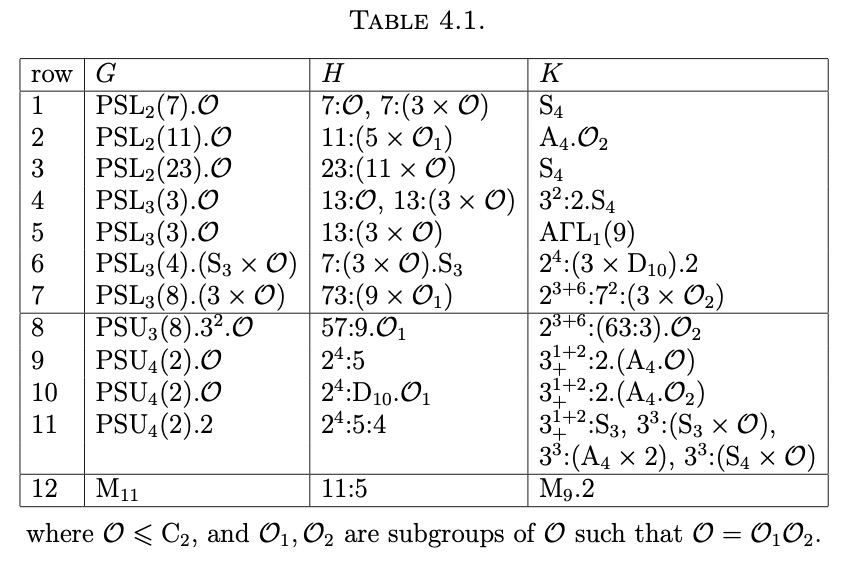
\includegraphics[width=9cm,height=6cm]{tab4.1.jpg}
\end{frame}

\begin{frame}
\begin{itemize}
	\item[1-3:] Excluded by lemma 5.1.
	\item[4-5:] $G=\PSL_3(3).2$, $G_\alpha=3^2:2.S_4$ or $\AGaL_1(9)\cong 3^2:8.2$\\  $G_\alpha^{\Gamma(\alpha)}$ 2-transitive$\implies \val(\Gamma)=\not 3,4,\not 9$. By ref.\footcite{LI2006164}, $G_\alpha=3^2:2.S_4$\\Hence $|V\Gamma|=26$, and \textcolor{blue}{$\Gamma=\PH(3,3^3)$} by ref.\footcite{CHENG1987196}\textsuperscript{, Table 1}.
	\item[6:] $G=\PSL_3(4).(S_3\times\mathbb{Z}_2)$ and $G_\alpha=2^4:(3\times D_{10}).2$\\3-arc-transitive$\implies \val(\Gamma)=5$, but $G_\alpha=\mathbb{Z}_4\times(\mathbb{Z}_5:\mathbb{Z}_4)$ by ref.\footcite{weiss_1979}
\end{itemize}
\underline{Claim:} If $\val(\Gamma)\geq 5$, then $|G_\alpha|$ divides $|G_\alpha^{\Gamma(\alpha)}|^2/\val(\Gamma)$.
\begin{itemize}
	\item[7:] $G=\PSU_3(8).(3\times \mathbb{Z}_2)$, $G_\alpha^{\Gamma(\alpha)}=2^3:7:3$, $\val(\Gamma)=8$, contradiction.
	\item[8:] $G=\PSU_3(8).3^2.2$, $G_\alpha^{\Gamma(\alpha)}=2^3:7:3$ with $\val(\Gamma)=2^3$ or $G_\alpha^{\Gamma(\alpha)}=2^6:63:3$ with $\val(\Gamma)=2^6$, both contradiction
	\item[9-11:] $G=\PSU_4(2)$, $G_\alpha=3^{1+2}_+:2.A_4$, $\val(\Gamma)=\not 4$(ref.\textsuperscript{15}),$\not 9$(3-arc-trans.)
	\item[12:] $G^+=M_{11}\implies G=M_{11}.2$ which is not in the table.
\end{itemize}
\end{frame}

\begin{frame}
\begin{lemma}[5.3]
T is not an alternating simple group.
\end{lemma}
\textbf{Proof. }Both $(G,H,G_\alpha)$ and $(G^+,H^+,G_\alpha)$ lie in the following. All possibilities can be excluded by lemma 2.3.

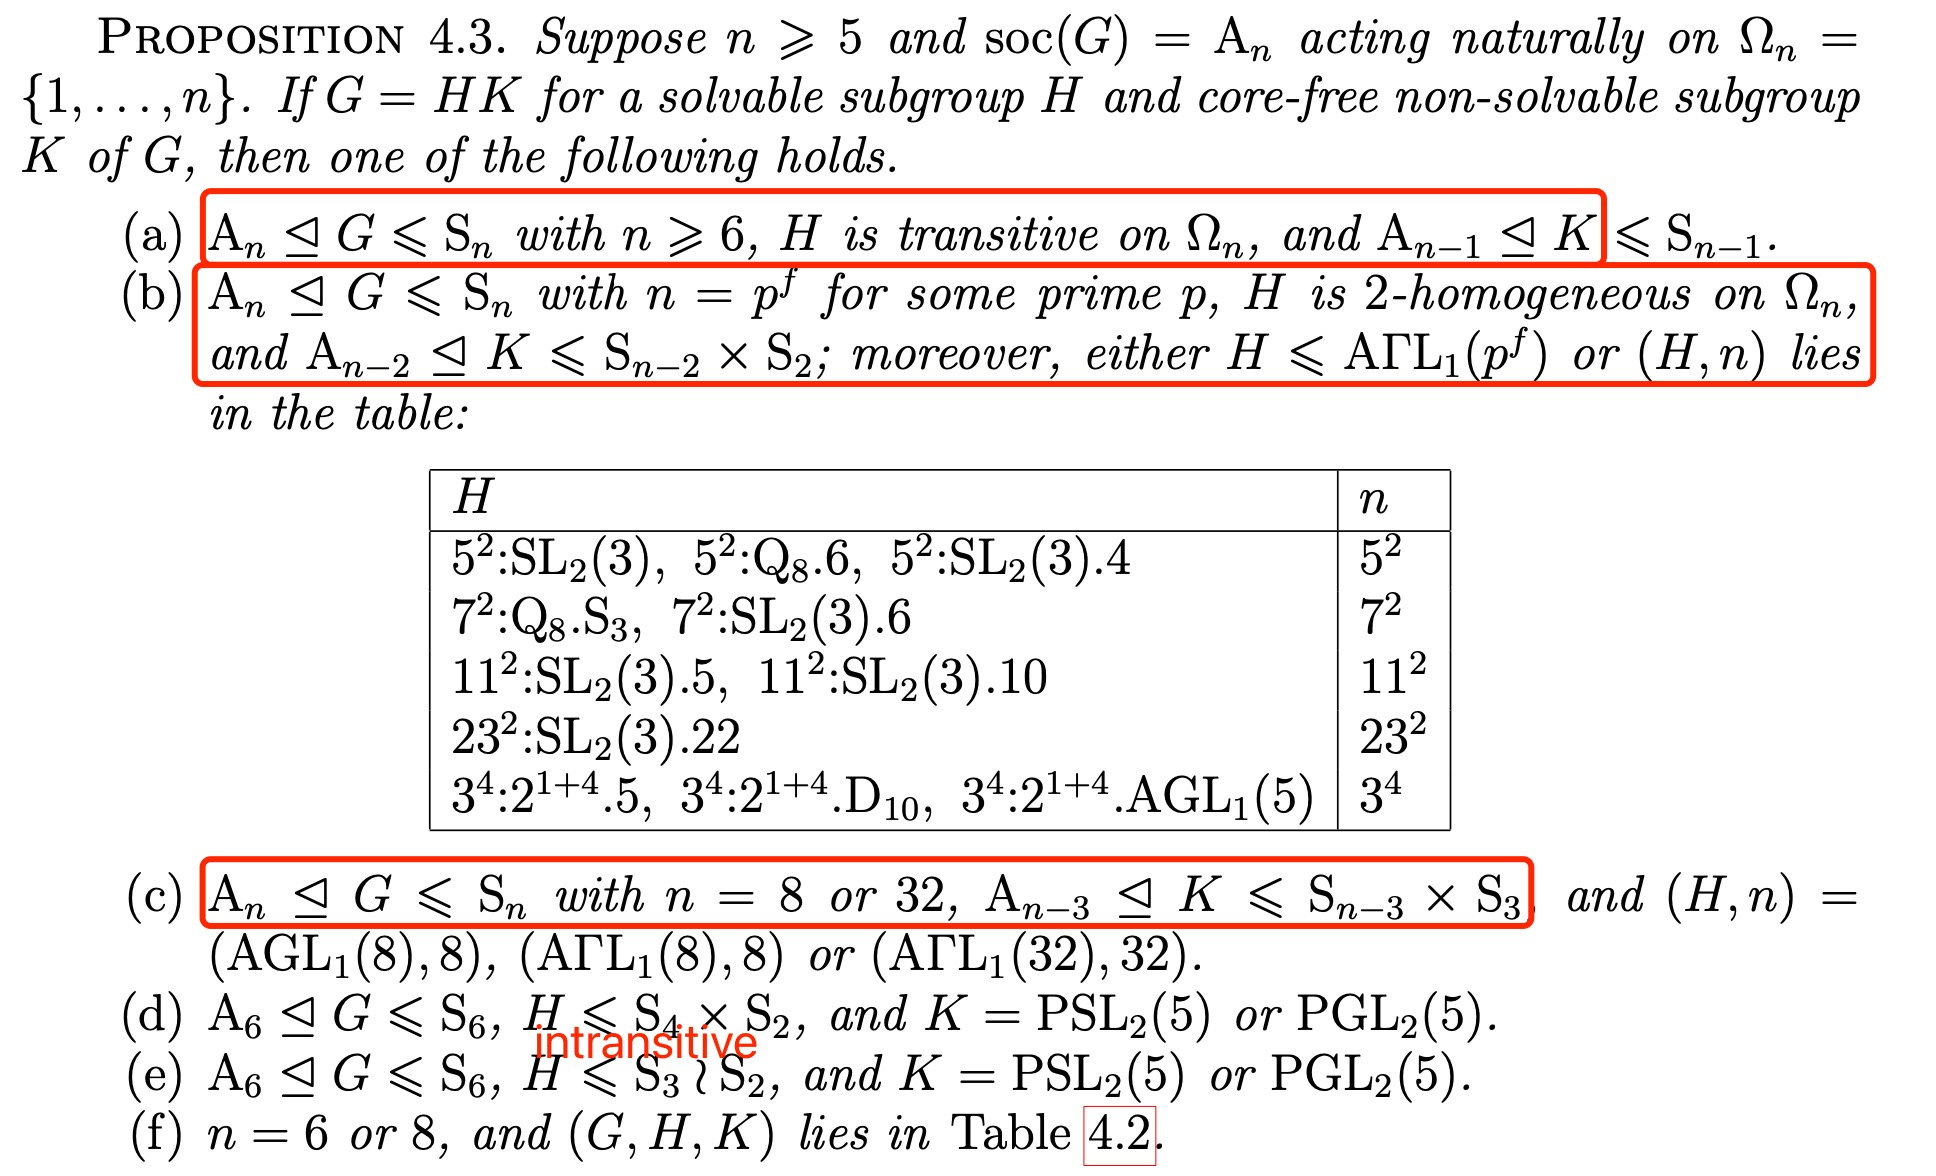
\includegraphics[width=6.5cm,height=5cm]{alternating.jpg}
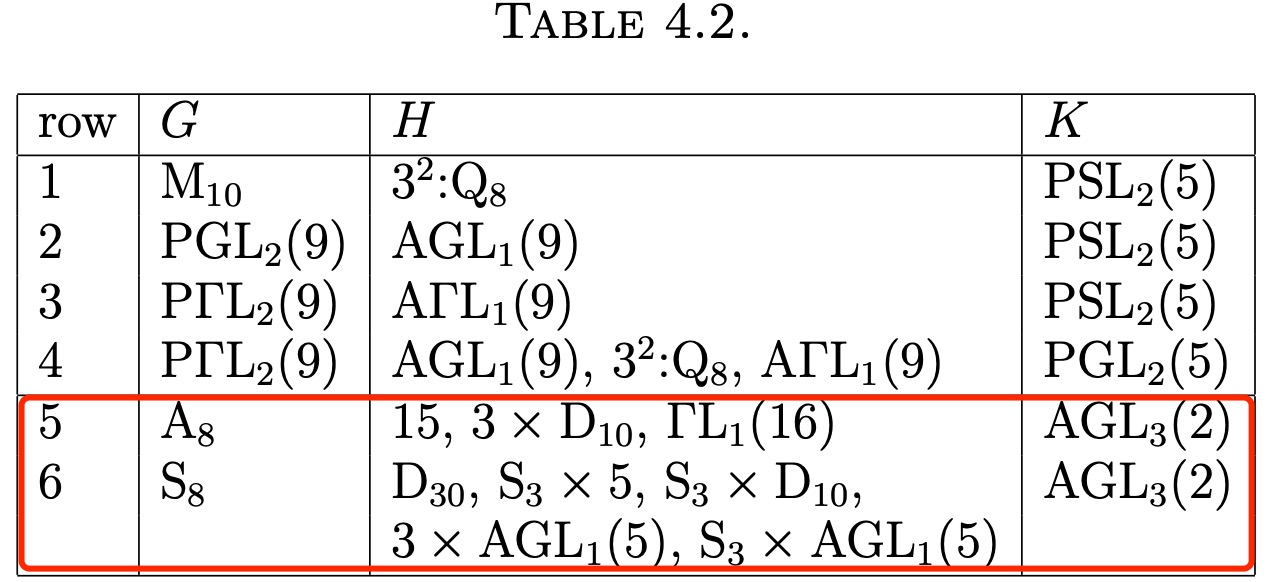
\includegraphics[width=4.3cm,height=3cm]{tab4.2.jpg}
\end{frame}

\begin{frame}
\begin{lemma}[5.4]
T is not a sporadic simple group.
\end{lemma}
\textbf{Proof. }Both $(G,H,G_\alpha)$ and $(G^+,H^+,G_\alpha)$ lie in the following.The only two possibilities can be excluded by lemma 2.3.
\center 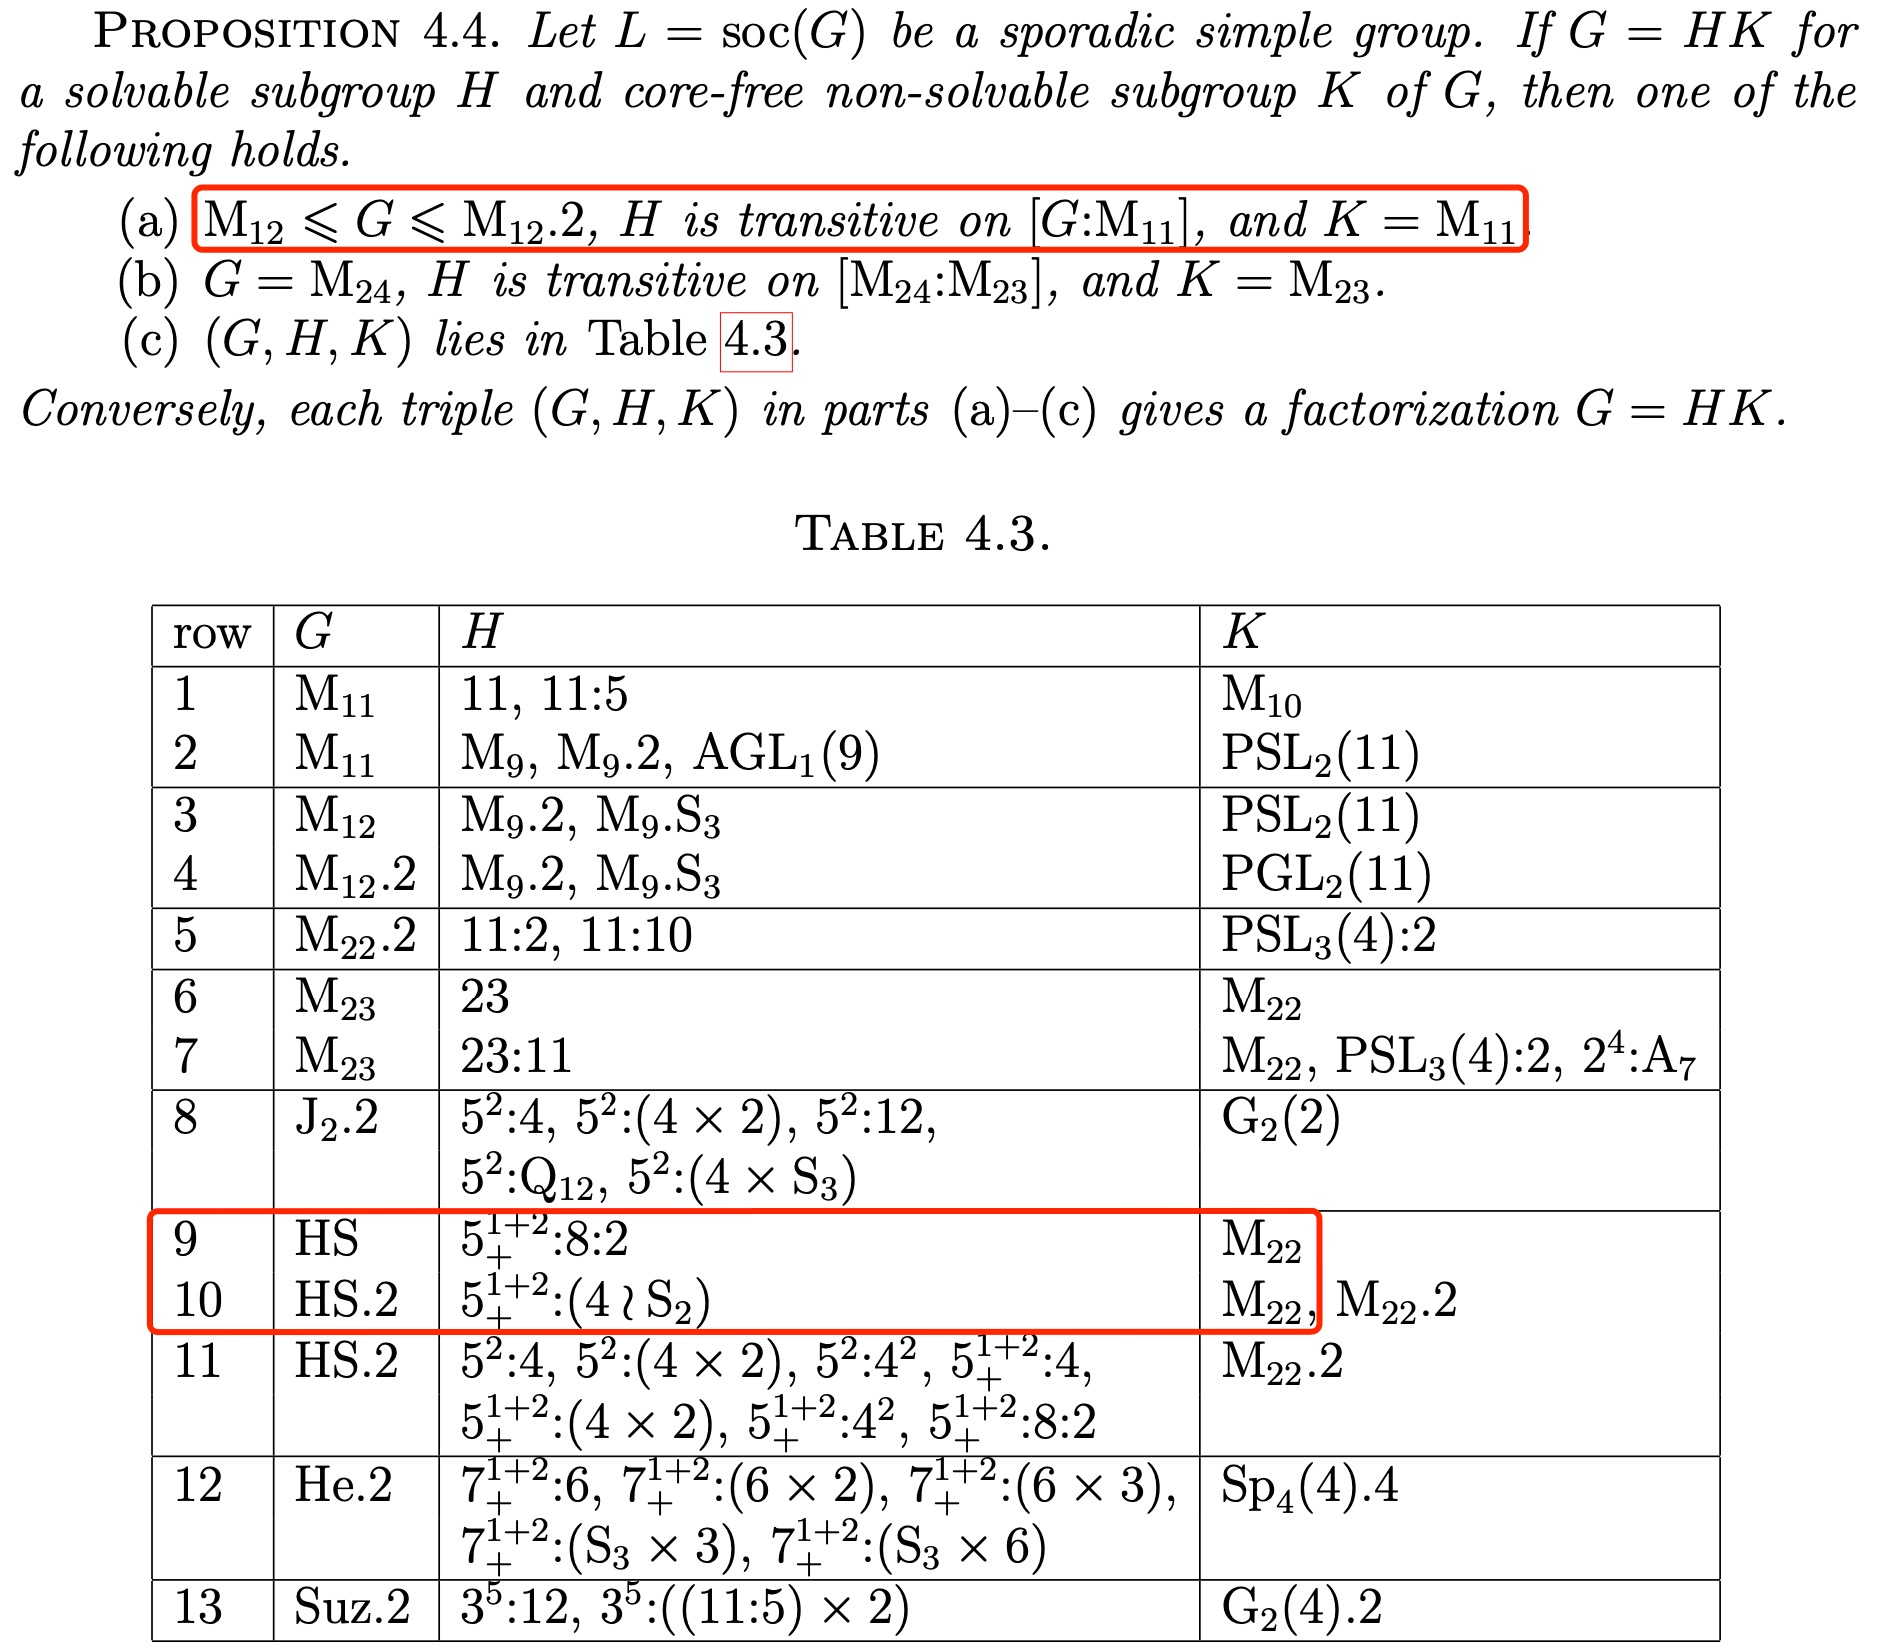
\includegraphics[width=7cm,height=6cm]{sporadical.jpg}
\end{frame}

\begin{frame}
\begin{lemma}[5.5]
If T is a classical simple group of Lie type, then $s\leq 4$, and one of the following is true.
\begin{enumerate}
	\item $T=\PSL_5(2)$, and $\Gamma\cong\GI(5,2,2)$.
	\item $T=\PSU_3(5)$, and $\Gamma\cong\HS_{50}^{(2)}$.
	\item $\Gamma$ is of valency $p^f+1$, $\PSL_3(p^f).2\leq G\leq\Aut(\PSL_3(p^f))$ and $\mathbb{Z}_p^{2f}:\SL_2(p^f)\triangleleft G_\alpha\leq P_1$ or $P_2$ where $P_1$ and $P_2$ are the stabilizers of T on a 1-dimension subspace and a 2-dimension subspace, respectively.
\end{enumerate}
\end{lemma}
\textbf{Proof. }If $G_\alpha$ solvable, then $T=\PSL_3(3)$, $\Gamma=\GI(3,1,3^3)$, satisfies (3).

If $G_\alpha$ is nonsolvable, note that $G_\alpha$ has a 2-transitive representation, hence has a minimal normal subgroup in the following list.\footcite{Cameron1981}
\end{frame}

\begin{frame}
\begin{center}
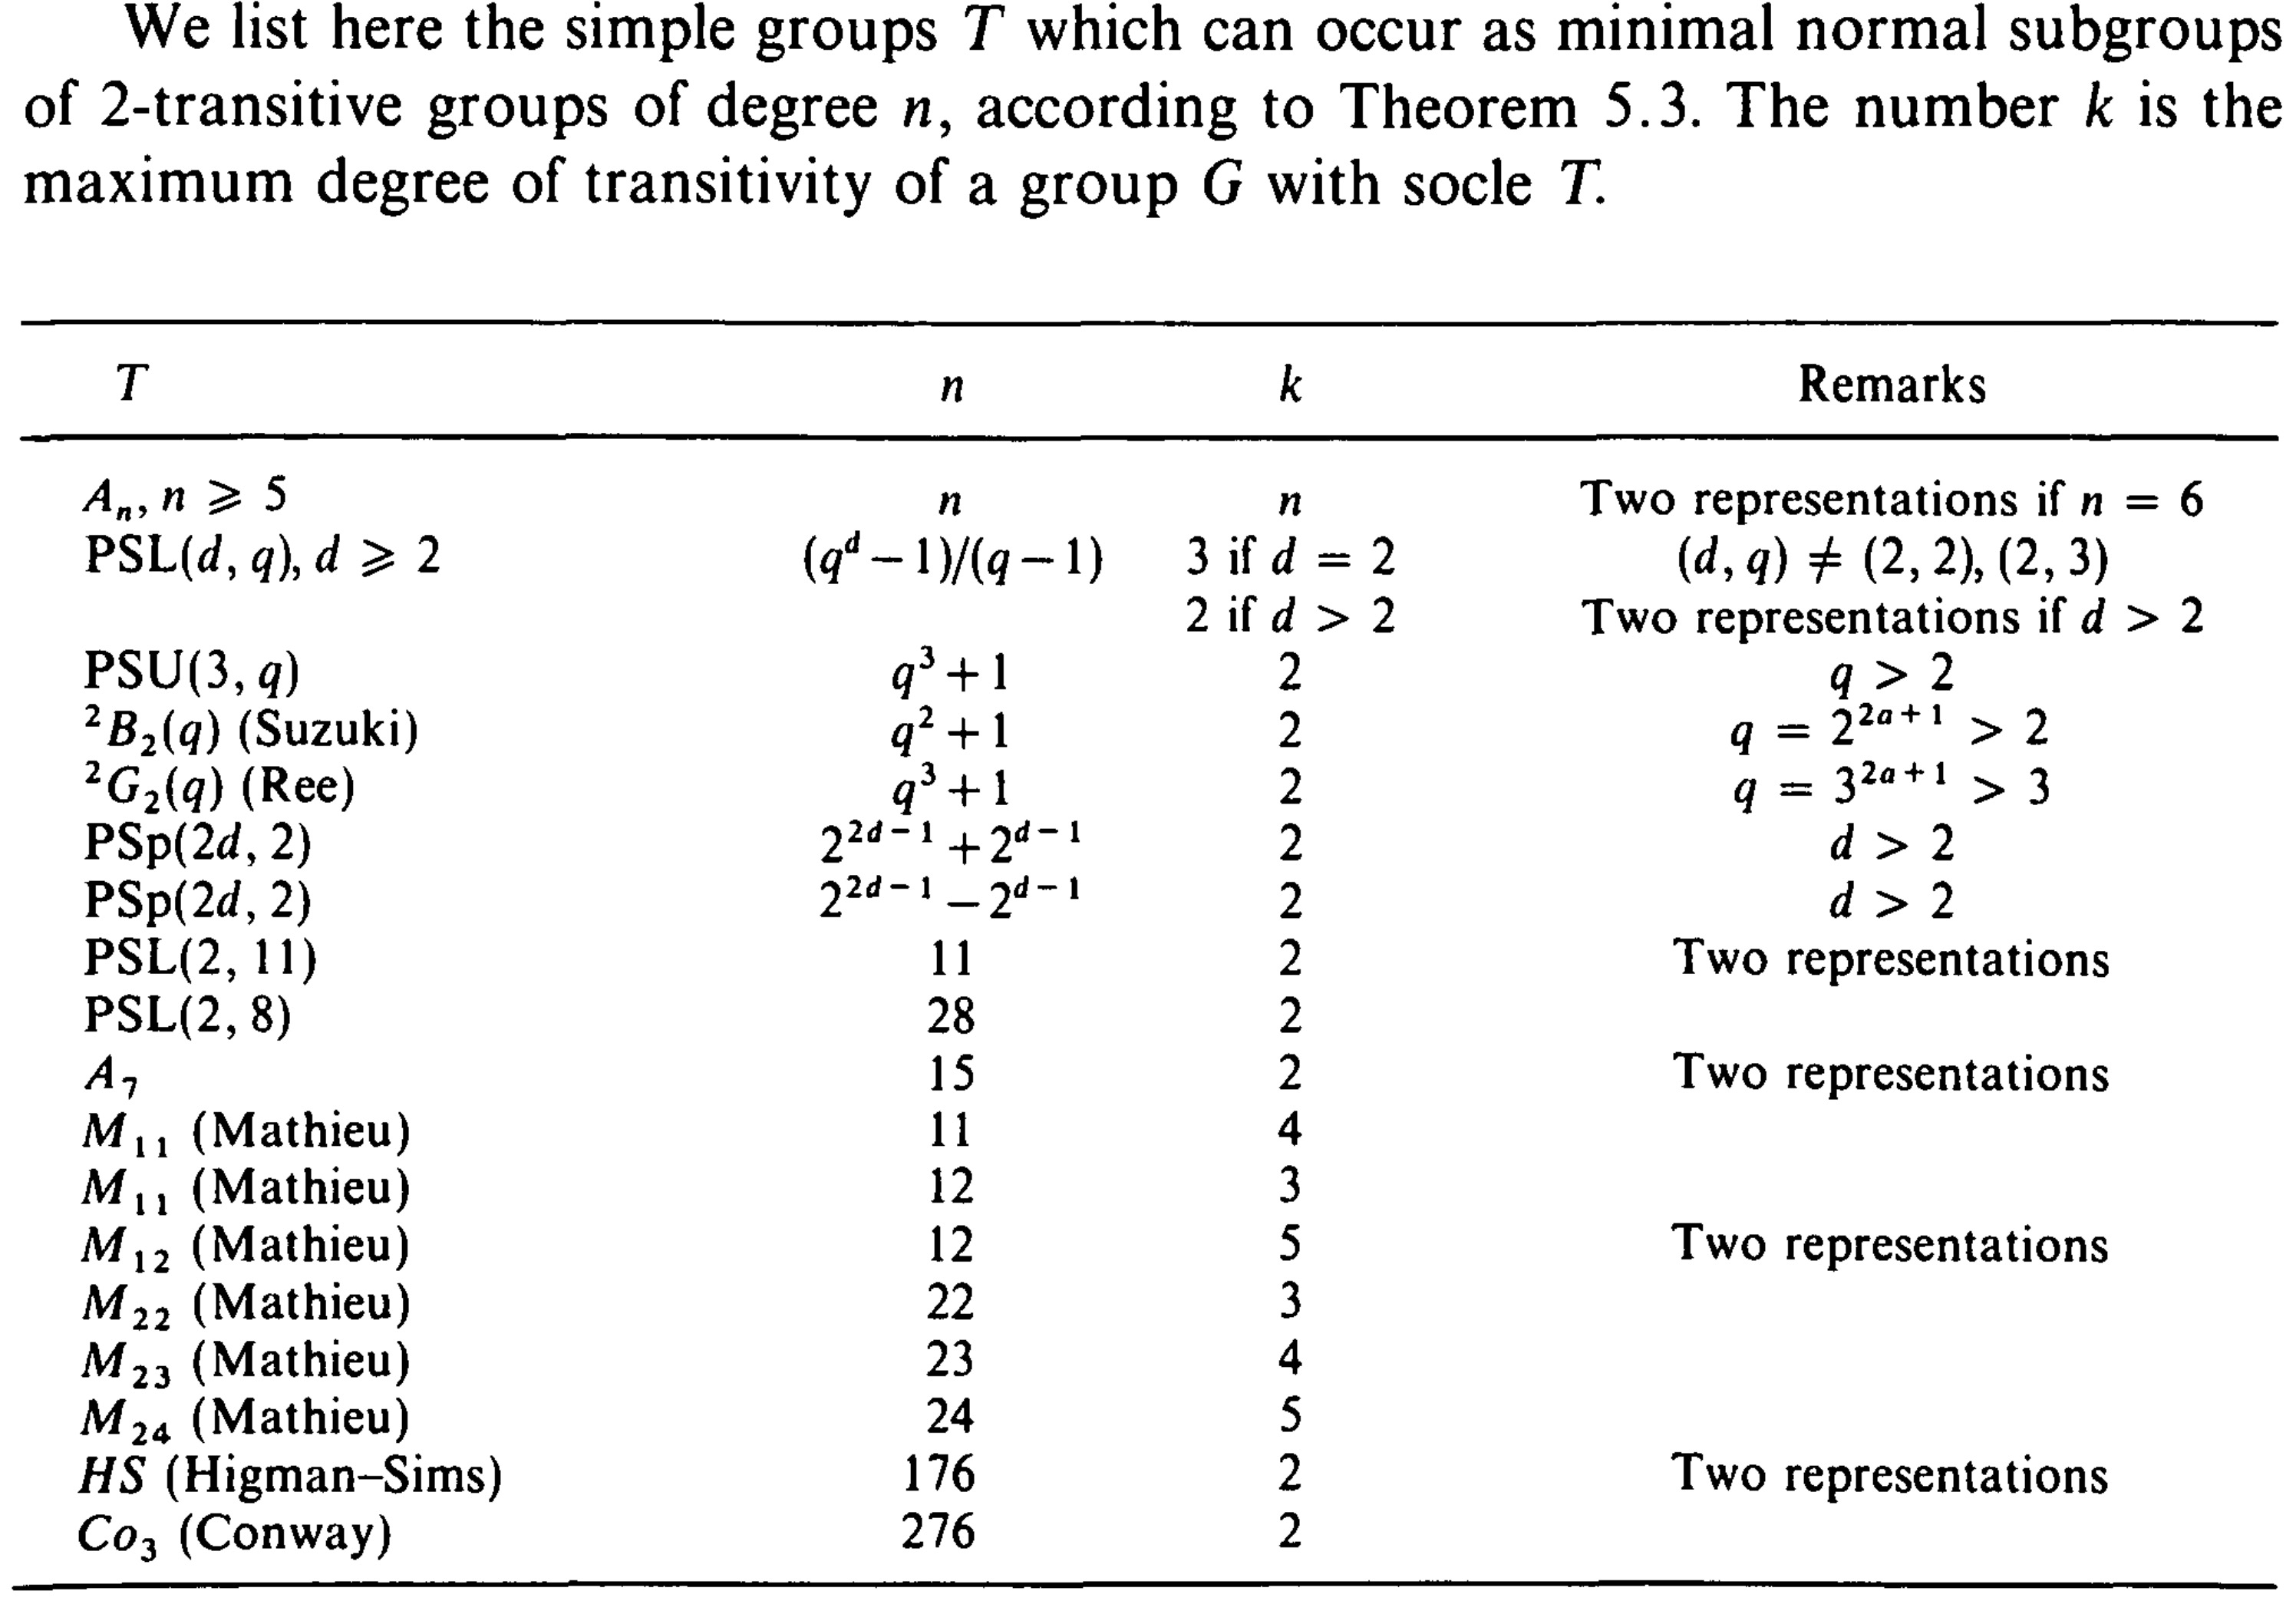
\includegraphics[width=8cm,height=6cm]{tab2-trans.jpg}
\end{center}
Notice that $1\neq T_\alpha\triangleleft G_\alpha$ and $T_\alpha\not\leq G_\alpha^{[1]}$.

Thus $T_\alpha$ has a composition factor listed above.
\end{frame}

\begin{frame}
Check $(T,H^+\cap T,T_\alpha)$ in following list.

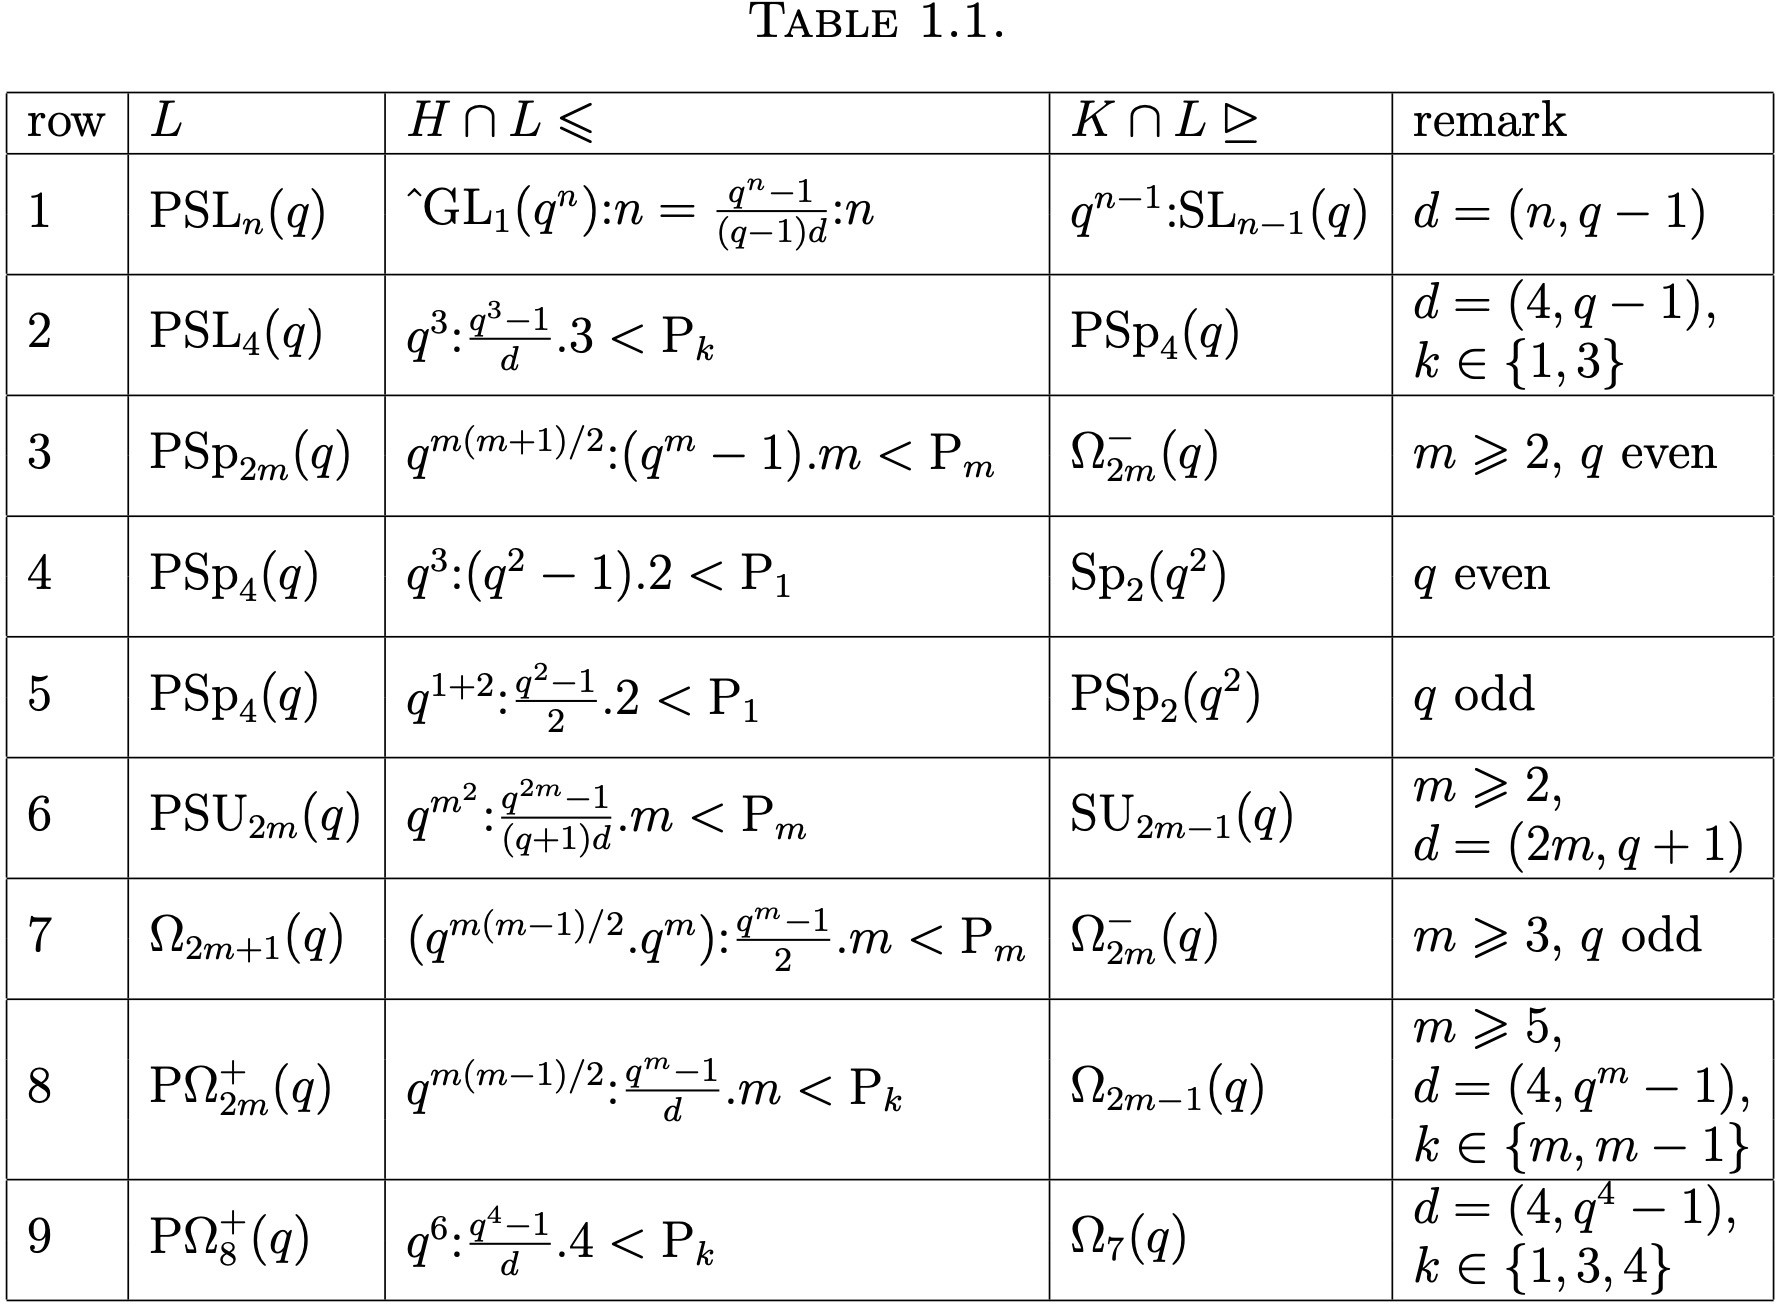
\includegraphics[width=6cm,height=6cm]{tab1.1.jpg}
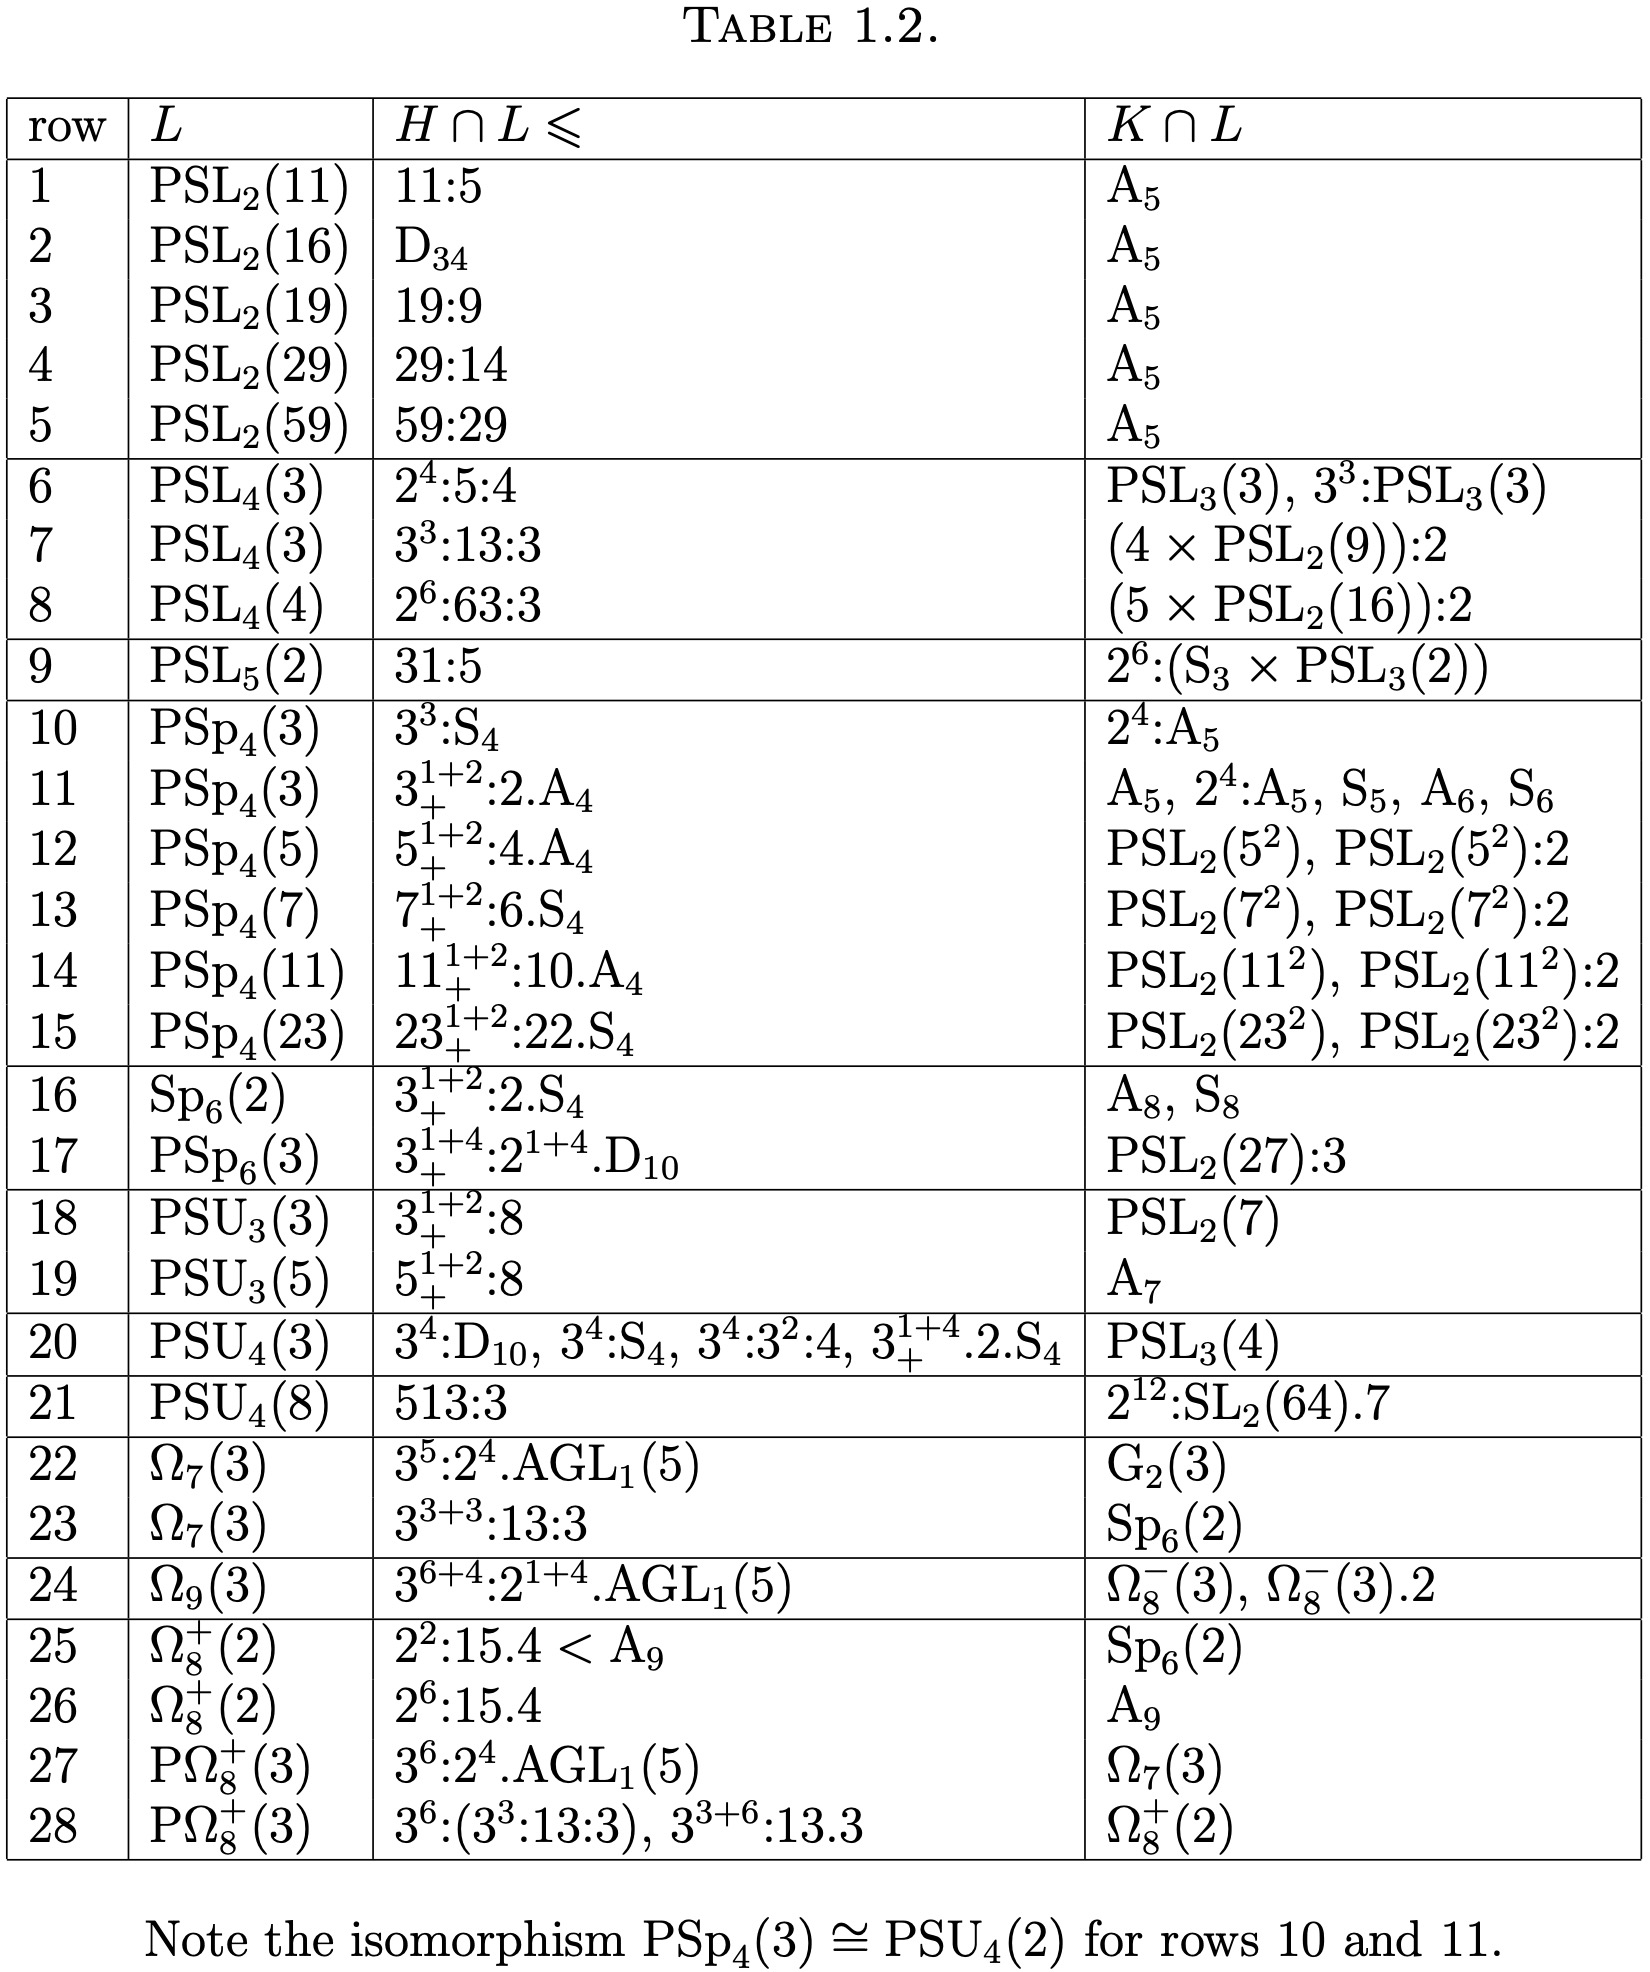
\includegraphics[width=5.5cm,height=7cm]{tab1.2.jpg}

\end{frame}

\begin{frame}
One of the following occurs:
\begin{enumerate}[(a)]
	\item $T=\PSL_n(p^f)$ and $\mathbb{Z}_p^{f(n-1)}:\SL_{n-1}(p^f)\triangleleft T_\alpha\leq P_1$ or $P_{n-1}$, where $n\geq 3$, $(n,p^f)\neq$ (3,2)  (3, 3) or (4, 2)
	\item $T=\PSp_4(p^f)$ and $\PSL_2(p^{2f})\triangleleft T_\alpha\triangleleft \PSL_2(p^{2f}).\mathbb{Z}_2$
	\item $T=\PSU_4(p^f)$, and $\PSU_3(p^f)\triangleleft T_\alpha$
	\item $(T,T\cap H^+,T_\alpha)$ lies in row 6-21, 23, 25-26 in Table 1.2
\end{enumerate}
\end{frame}

\begin{frame}
\textbf{Case (a):}

If $G_\alpha^{\Gamma(\alpha)}$ is affine, then ref.\footcite{Cameron_1999}\textsuperscript{,Table7.3} implies contradiction.

Thus $G_\alpha^{\Gamma(\alpha)}$ is AS with socle $\PSL_{n-1}(p^f)$, and $\val(\Gamma)=\frac{p^{f(n-1)}-1}{p^f-1}$.
\[ \val(\Gamma)-1\text{ divides } |G_\alpha^{[1]}|\text{ divides }\frac{|P_1||\Out(T)|}{2|\PSL_{n-1}(p^f)|}=fp^{f(n-1)}(p^f-1). \]
Thus $p^{f(n-2)}-1$ divides $fp^{f(n-2)}(p^f-1)^2$.

\ 

Now $n\geq 4$ implies $p^{f(n-2)}-1$ has a ppd r, while r divides the left but not right side of above formula. A contradicition.

\ 

Thus $n=3$, $\val(\Gamma)=p^f+1$ and $\mathbb{Z}_p^{2f}:\SL_2(p^f)\triangleleft G_\alpha$.

So $s\leq 4$ by Theorem 2.2.

\end{frame}


\begin{frame}
\textbf{Case (b):} $G_\alpha^{\Gamma(\alpha)}$ is almost simple with socle $\PSL_2(p^{2f})$, \textcolor{red}{$\val(\Gamma)=p^{2f}+1$, }
\[|G_\alpha^{[1]}|\text{ divides }\frac{|G_\alpha|}{G_\alpha^{\Gamma(\alpha)}}=\frac{|T_\alpha||\mathcal{O}'|}{G_\alpha^{\Gamma(\alpha)}}\text{ divides }2|\mathcal{O}'|\text{ divides }|\Out(\PSp_4(p^f))|=2f\]
However, by lemma 2.3, $p^{2f}=\val(\Gamma)-1$ divides $|G_\alpha^{[1]}|$. A contradiction.


\ 

\textbf{Case (c):} Similar as above, \[p^{3f}=\val(\Gamma)-1\text{ divides }|\Out(T)|/2=f(4,p^f+1).\]
\end{frame}


\begin{frame}
\textbf{Case (d):}
\begin{itemize}\setlength{\itemindent}{1em}
	\item[row 6-8:] MAGMA shows no such graph
	\item[row 9:] $T=\PSL_5(2)$, $T_\alpha=2^6:(S_3\times \PSL_3(2))$. \textcolor{blue}{Example(2): $\GI(5,2,2)$.}
	\item[row 19:] $T=\PSU_3(5)$, $T_\alpha=A_7$. \textcolor{blue}{Example(3): $\HS_{50}^{(2)}$.}
	\item[row 20:] $T=\PSU_4(3)$, $T_\alpha=\PSL_3(4)$, $\val(\Gamma)=21$. \\But $|\Out(T)|=8$ not divisible by $\val(\Gamma)-1$.
	\item[row 21:] $T=\PSU_4(8)$, $T_\alpha=\mathbb{Z}_2^{12}:\SL_2(64).\mathbb{Z}_7$, $\Out(T)=\mathbb{Z}_6$.\\By ref.\footcite{Cameron_1999}\textsuperscript{,Table7.3}, $G_\alpha^{\Gamma(\alpha)}$ is AS with socle $\PSL_2(64)$ and $\val(\Gamma)=65$. \\MAGMA shows no such graph.
	\item[else:] $T_\alpha$ is AS with $\soc(T_\alpha)\neq A_7$, $|\Out(T)|<8$. \textcolor{red}{$|G_\alpha^{[1]}|$ divides $\frac{|\Out(T)|}{2}$.}\\But nonsolvable $G_\alpha$ implies $\val(\Gamma)\geq 5$. A contradiction.
\end{itemize}

\end{frame}



%%%%%%%%%%%%%%%%%%%%%%%%%%%%%%%



\begin{frame}{References}
\tiny
\printbibliography
\end{frame}



\end{document}


